\documentclass[12pt,a4paper,twoside,openright]{report}
% Compile with XeLaTeX or LuaLaTeX (fontspec + Greek abstract require Unicode engines).

% ============================================================================
% PACKAGES
% ============================================================================
\usepackage{fontspec}
\usepackage{polyglossia}
% NTUA-style thesis formatting (see department guidelines)
% - Body: 11--12pt Times New Roman (Arial fallback)
% - Headings: 14--16pt
% - Line spacing: 1.5
% - Alignment: justified

% Main font: Times New Roman, fallback Arial
\IfFontExistsTF{Times New Roman}
  {\setmainfont{Times New Roman}[Ligatures=TeX]}
  {\IfFontExistsTF{Arial}
    {\setmainfont{Arial}[Ligatures=TeX]}
    {\setmainfont{TeX Gyre Termes}[Ligatures=TeX]}}

\IfFontExistsTF{Arial}
  {\setsansfont{Arial}[Ligatures=TeX]}
  {\setsansfont{TeX Gyre Heros}[Ligatures=TeX]}

% Justified body text
\usepackage{microtype}
\usepackage{ragged2e}
\justifying

% Heading sizes (14--16pt range) without titlesec
\makeatletter
\renewcommand\@makechapterhead[1]{%
  \vspace*{50\p@}%
  {\parindent \z@ \raggedright \normalfont
    \ifnum \c@secnumdepth >\m@ne
      {\bfseries\fontsize{16}{24}\selectfont
        \chaptername\space \thechapter\par\nobreak\vskip 12\p@}%
    \fi
    \interlinepenalty\@M
    \bfseries\fontsize{16}{24}\selectfont #1\par\nobreak
    \vskip 32\p@}}

\renewcommand\@makeschapterhead[1]{%
  \vspace*{50\p@}%
  {\parindent \z@ \raggedright
    \interlinepenalty\@M
    \bfseries\fontsize{16}{24}\selectfont #1\par\nobreak
    \vskip 32\p@}}

\renewcommand\section{%
  \@startsection{section}{1}{\z@}%
    {-3.5ex \@plus -1ex \@minus -.2ex}%
    {2.3ex \@plus .2ex}%
    {\normalfont\bfseries\fontsize{14}{21}\selectfont}}

\renewcommand\subsection{%
  \@startsection{subsection}{2}{\z@}%
    {-3.25ex\@plus -1ex \@minus -.2ex}%
    {1.5ex \@plus .2ex}%
    {\normalfont\bfseries\fontsize{14}{21}\selectfont}}

\renewcommand\subsubsection{%
  \@startsection{subsubsection}{3}{\z@}%
    {-3.25ex\@plus -1ex \@minus -.2ex}%
    {1.5ex \@plus .2ex}%
    {\normalfont\bfseries\fontsize{12}{18}\selectfont}}
\makeatother

% Running head (title) and footer (author); page numbers at bottom outer edge
\providecommand{\thesisrunningtitle}{Modeling Smart Electric Vehicle Charging}
\providecommand{\thesisauthor}{Christos Kontomitros}

\usepackage{fancyhdr}
\setlength{\headheight}{14.5pt}
\addtolength{\topmargin}{-2.5pt}
\pagestyle{fancy}
\fancyhf{}
\fancyhead[CE,CO]{\small\thesisrunningtitle}
\fancyfoot[C]{\small\thesisauthor}
\fancyfoot[LE,RO]{\thepage}
\renewcommand{\headrulewidth}{0.4pt}
\renewcommand{\footrulewidth}{0pt}

\fancypagestyle{plain}{%
  \fancyhf{}%
  \fancyhead[CE,CO]{\small\thesisrunningtitle}%
  \fancyfoot[C]{\small\thesisauthor}%
  \fancyfoot[LE,RO]{\thepage}%
  \renewcommand{\headrulewidth}{0.4pt}%
}

\setdefaultlanguage{english}
\setotherlanguage{greek}
% Greek body text must use a font that actually contains Greek letters (the Latin default often does not).
% Prefer a system/office font; fall back for typical Linux installs. Install fonts or texlive-fontsextra if needed.
\IfFontExistsTF{Times New Roman}
  {\newfontfamily\greekfont{Times New Roman}[Ligatures=TeX,Scale=MatchLowercase]}
  {\IfFontExistsTF{Liberation Serif}
    {\newfontfamily\greekfont{Liberation Serif}[Ligatures=TeX,Scale=MatchLowercase]}
    {\newfontfamily\greekfont{DejaVu Serif}[Ligatures=TeX,Scale=MatchLowercase]}}
\newenvironment{greekabstract}{\begin{greek}}{\end{greek}}

% Math packages
\usepackage{amsmath}
\usepackage{amssymb}
\usepackage{amsthm}

% Graphics and figures
\usepackage{graphicx}
\usepackage{subfig}
\usepackage{float}
\usepackage{caption}

% Tables
\usepackage{booktabs}
\usepackage{multirow}
\usepackage{array}

% Code listings
\usepackage{listings}
\usepackage{xcolor}

% Algorithms
\usepackage{algorithm}
\usepackage{algpseudocode}

% References and citations
\usepackage[style=ieee,backend=bibtex]{biblatex}
\addbibresource{references.bib}

% Hyperlinks
\usepackage[colorlinks=true,linkcolor=blue,citecolor=blue,urlcolor=blue]{hyperref}

% Page layout
\usepackage[inner=3cm,outer=2.5cm,top=2.5cm,bottom=2.5cm]{geometry}
\usepackage{setspace}
\onehalfspacing

% Custom commands
\newcommand{\soc}{\text{SoC}}
\newcommand{\ev}{\text{EV}}
\newcommand{\kwh}{\text{kWh}}
\newcommand{\kw}{\text{kW}}

% Code listing style
\lstset{
    basicstyle=\ttfamily\small,
    keywordstyle=\color{blue},
    commentstyle=\color{gray},
    stringstyle=\color{red},
    numbers=left,
    numberstyle=\tiny\color{gray},
    stepnumber=1,
    numbersep=8pt,
    showstringspaces=false,
    breaklines=true,
    frame=single,
    captionpos=b
}

% ============================================================================
% DOCUMENT
% ============================================================================
\begin{document}

% ----------------------------------------------------------------------------
% FRONT MATTER
% ----------------------------------------------------------------------------
% ============================================================================
% FRONT MATTER
% ============================================================================

% Title page
\begin{titlepage}
    \centering
    \vspace*{1cm}
    
    % University logo (add your logo file)
    % \includegraphics[width=0.3\textwidth]{figures/university_logo.png}\\[1cm]
    
    {\LARGE \textbf{National Technical University of Athens}}\\[0.5cm]
    {\large School of Electrical and Computer Engineering}\\[2cm]
    
    {\huge \textbf{Modeling Smart Electric Vehicle Charging}}\\[0.5cm]
    {\Large \textbf{A Multi-Level Intelligence Approach with Renewable Energy Integration}}\\[3cm]
    
    {\large \textbf{Diploma Thesis}}\\[1cm]
    
    {\large by}\\[0.5cm]
    {\Large \textbf{Christos Kontomitros}}\\[2cm]
    
    {\large Supervisor: Prof. Alexandros Flamos}\\[0.2cm]
    {\large Co-supervisor: Dr. Dimitris Fotopoulos }\\[3cm]
    
    {\large Piraeus, April 2026}
    
\end{titlepage}

% Abstract (Greek)
\chapter*{Περίληψη}
\addcontentsline{toc}{chapter}{Περίληψη}

[Γράψε εδώ την περίληψη στα ελληνικά - 300-500 λέξεις]

Η παρούσα διπλωματική εργασία διερευνά την εφαρμογή έξυπνων συστημάτων φόρτισης ηλεκτρικών οχημάτων σε κτίρια γραφείων με ενσωμάτωση ανανεώσιμων πηγών ενέργειας. Αναλύονται διαφορετικά επίπεδα "ευφυίας" από απλούς κανόνες έως προηγμένους αλγορίθμους βελτιστοποίησης και τεχνολογία Vehicle-to-Grid (V2G)...

\textbf{Λέξεις κλειδιά:} Ηλεκτρικά οχήματα, έξυπνη φόρτιση, ανανεώσιμες πηγές ενέργειας, βελτιστοποίηση, Vehicle-to-Grid, κτίρια γραφείων

\newpage

% Abstract (English)
\chapter*{Abstract}
\addcontentsline{toc}{chapter}{Abstract}

[Write your abstract in English - 300-500 words]

This diploma thesis investigates the application of smart electric vehicle (EV) charging systems in office buildings with renewable energy integration. Different levels of intelligence are analyzed, ranging from simple rule-based approaches to advanced optimization algorithms and Vehicle-to-Grid (V2G) technology...

\textbf{Keywords:} Electric vehicles, smart charging, renewable energy, optimization, Vehicle-to-Grid, office buildings

\newpage

% Acknowledgments
\chapter*{Acknowledgments}
\addcontentsline{toc}{chapter}{Acknowledgments}

[Write your acknowledgments here]

I would like to express my sincere gratitude to my supervisors Alexandros Flamos and Dimitris Fotopoulos for their guidance and support throughout this research...

\newpage

% ============================================================================
% LIST OF ABBREVIATIONS
% ============================================================================

\chapter*{List of Abbreviations}
\addcontentsline{toc}{chapter}{List of Abbreviations}

\begin{tabular}{@{}>{\bfseries}p{2.8cm}p{11.2cm}@{}}
ANN & Artificial Neural Network \\
DDPG & Deep Deterministic Policy Gradient \\
DQN & Deep Q-Network \\
DRL & Deep Reinforcement Learning \\
ELMAS & European Load Model for Aggregated Sectors \\
ESS & Energy Storage System \\
EV & Electric Vehicle \\
kW & Kilowatt \\
kWh & Kilowatt-hour \\
MADRL & Multi-Agent Deep Reinforcement Learning \\
MPC & Model Predictive Control \\
PERC & Passivated Emitter and Rear Cell \\
PV & Photovoltaic \\
PVGIS & Photovoltaic Geographical Information System \\
RES & Renewable Energy Source \\
RL & Reinforcement Learning \\
SARAH3 & Surface Solar Radiation Data Set (PVGIS database) \\
SoC & State of Charge \\
STC & Standard Test Conditions \\
V2G & Vehicle-to-Grid \\
Wp & Watt-peak (rated module power) \\
\end{tabular}

\newpage


% Table of contents
\tableofcontents
\listoffigures
\listoftables

% ----------------------------------------------------------------------------
% MAIN CONTENT
% ----------------------------------------------------------------------------
% ============================================================================
% CHAPTER 1: INTRODUCTION
% ============================================================================
\chapter{Introduction}
\label{ch:introduction}

\section{Background and Motivation}
\label{sec:background}

Recent climate regulations have led to a rise in the adoption of electric vehicles. More and more people are opting for an electric vehicle for their daily commute. According to studies, most of the time spent in commute is on the way to and from the office. Also, most people spend a third of their time in offices, and with them their cars, 
which can be charged during the workday. The car batteries can also be used in times of peak consumption to give electricity back to the building or to the grid. Since the charging will happen throughout the day,  
it is logical to create smart charging algorithms that can utilise information from solar power generation, pricing spreads throughout the day, and grid capacity limits in order to optimise the charging schedule. Office buildings also offer a huge rooftop space for the installation of solar panels; 
the energy produced by these panels can be used both for the building's consumption as well as for the charging of the electric vehicles. The cost of electricity produced is zero, and this helps reduce the overall cost. As such, the utilization of renewable energy is the most important aspect of the charging algorithm. 

\section{Literature Review}
\label{sec:literature_review}

Currently, there are many different algorithms that are used for the smart scheduling of the EV fleet. Early studies, such as Richardson \cite{richardson2012ev_ucd}, used linear programming in order to decide which vehicle will be charged and when in 15-minute intervals,
taking into account network limitations. Further studies included the use of reinforcement learning to increase grid stability, and optimize for pricing and renewables utilization; several studies are included in this review \cite{qiu2023rl_ev_review}.

\section{Smart Charging Levels}
\label{sec:smart_charging_levels}

The algorithms developed in this thesis are separated by their intelligence levels. Level 0 is a simple rule-based algorithm that prioritises solar renewable energy, respecting grid constraints and the target charging SOC of the EV battery; it charges without respecting future price levels. 
Level 1 is a Q-learning algorithm that uses a reward function to include information about price levels and also the availability of solar energy. Level 2 is a Q-learning algorithm that also includes the action of discharging energy back to the grid. The remaining chapters focus on different parts of the algorithms.

\section{Thesis Structure}
\label{sec:structure}

Chapter~2 focuses more on the models that describe the office, the EVs, the grid, and the solar panels. Chapter~3 focuses on the data for the office building consumption, electricity pricing, and solar generation. Chapter~4 focuses on the simulation using each algorithm, collecting and comparing the results.
Chapter~5 focuses on the conclusion of the results and recommendations for future work.
% ============================================================================
% CHAPTER 2: METHODOLOGY
% ============================================================================
\chapter{Methodology}
\label{ch:methodology}

This chapter presents the mathematical models and algorithms used to simulate and optimize EV charging in office buildings. We describe the system components, optimization objectives, and the specific implementation of each intelligence level.

\section{System Components}
\label{sec:system_components}

\subsection{Office Building Model}
\label{subsec:building_model}

The office building is characterized by its energy consumption and renewable generation profiles.

\subsubsection{Energy Consumption}

The building's hourly energy consumption profile $C_b(t)$ is derived from the ELMAS dataset (European Load Model for Aggregated Sectors), specifically the Office cluster (\#5) from \texttt{Time\_series\_18\_clusters.csv}.

Let $L_t$ denote the hourly load of the Office cluster base series ($T = 8{,}736$ hours for year 2018) with annual energy:

\begin{equation}
E_{cluster} = \sum_{t=1}^{T} L_t
\end{equation}

To determine a representative single-building target, the per-customer annual energy is computed for each class $c$ belonging to the Office cluster:

\begin{equation}
e_c = \frac{E_c}{N_c}
\end{equation}

where $E_c$ is the annual energy and $N_c$ the number of customers in class $c$. The target annual energy is set to the 75th percentile of the per-customer distribution:

\begin{equation}
E_{target} = Q_{0.75}\!\left(\{e_c\}\right) = 58{,}831 \; \text{\kwh}
\end{equation}

The cluster profile is then scaled to match this target:

\begin{equation}
L_t^{scaled} = L_t \cdot \frac{E_{target}}{E_{cluster}}
\end{equation}

To introduce realistic stochastic variability, two multiplicative noise factors are applied---a daily factor $\alpha_d$ (constant within each day) and an hourly factor $\beta_t$:

\begin{align}
\alpha_d &\sim \mathcal{N}(1, \sigma_d^2), \quad \sigma_d = 0.08, \quad \alpha_d \in [0.7, 1.3] \\
\beta_t &\sim \mathcal{N}(1, \sigma_h^2), \quad \sigma_h = 0.03, \quad \beta_t \in [0.9, 1.1]
\end{align}

The synthetic series before re-normalization:

\begin{equation}
L_t^{syn} = L_t^{scaled} \cdot \alpha_d(t) \cdot \beta_t
\end{equation}

Finally, the series is re-scaled to exactly preserve the target annual energy:

\begin{equation}
C_b(t) = L_t^{syn} \cdot \frac{E_{target}}{\sum_{t=1}^{T} L_t^{syn}}
\label{eq:building_consumption}
\end{equation}

The resulting single-office profile has a mean load of 6.73~\kw{} and a peak load of 11.92~\kw.

\subsubsection{Solar Photovoltaic System}

The solar PV system generates electricity based on irradiance:

\begin{equation}
P_{solar}(t) = A_{panel} \cdot \eta_{panel} \cdot I(t)
\end{equation}

where:
\begin{itemize}
    \item $A_{panel}$ = solar panel area (m²)
    \item $\eta_{panel}$ = panel efficiency
    \item $I(t)$ = solar irradiance at hour $t$ (W/m²)
\end{itemize}

\subsubsection{Building Battery Storage}

The building includes a stationary battery with capacity $C$ and state of charge $\soc_b(t)$.

The maximum discharge power at time $t$ is bounded by both the inverter rating and the available energy above the minimum SoC:

\begin{equation}
P_{dis,t} = \min\!\left( P_{max}, \; (\soc_{t-1} - \soc_{min}) \cdot \eta \right)
\label{eq:battery_discharge_power}
\end{equation}

Similarly, the maximum charge power is limited by the inverter and the remaining capacity:

\begin{equation}
P_{ch,t} = \min\!\left( P_{max}, \; C - \soc_{t-1} \right)
\label{eq:battery_charge_power}
\end{equation}

The state of charge evolves depending on whether the building has excess or missing energy. When excess solar energy is available, the battery charges:

\begin{equation}
\soc_t = \soc_{t-1} + \min\!\left( P_{ch,t}, \; E_{excess}(t) \right)
\label{eq:soc_charge}
\end{equation}

When the building demand exceeds supply, the battery discharges:

\begin{equation}
\soc_t = \soc_{t-1} - \min\!\left( \frac{P_{dis,t}}{\eta}, \; \frac{E_{missing}(t)}{\eta} \right)
\label{eq:soc_discharge}
\end{equation}

where:
\begin{itemize}
    \item $P_{max}$ = maximum charge/discharge power [\kw]
    \item $C$ = battery capacity [\kwh]
    \item $\soc_{min}$ = minimum allowable state of charge
    \item $\eta$ = round-trip efficiency
    \item $E_{excess}(t) = \max(0, \; P_{solar}(t) - C_b(t))$ = surplus solar energy
    \item $E_{missing}(t) = \max(0, \; C_b(t) - P_{solar}(t))$ = energy deficit
\end{itemize}

Constraints:
\begin{align}
\soc_{min} &\leq \soc_t \leq C \\
0 &\leq P_{ch,t} \leq P_{max} \\
0 &\leq P_{dis,t} \leq P_{max}
\end{align}

\subsubsection{Net Energy Demand}

The building's net energy demand (positive = needs grid, negative = surplus):

\begin{equation}
E_{net}^{building}(t) = C_b(t) - P_{solar}(t) - E_{discharge}^b(t) + E_{charge}^b(t)
\end{equation}

\subsection{Electric Vehicle Fleet Model}
\label{subsec:ev_model}

\subsubsection{Individual EV Characteristics}

Each EV $i$ in the fleet is characterized by:

\begin{itemize}
    \item Battery capacity: $B_{cap}^{i}$ [\kwh]
    \item State of charge: $\soc^i(t)$ [dimensionless, 0-1]
    \item Maximum charge rate: $P_{max,charge}^{i}$ [\kw]
    \item Maximum discharge rate: $P_{max,discharge}^{i}$ [\kw] (for V2G)
    \item Arrival time: $t_{arrival}^{i}$ [hour]
    \item Departure time: $t_{target}^{i}$ [hour]
    \item Desired SoC: $\soc_{desired}^{i}$ [dimensionless]
\end{itemize}

\subsubsection{EV Battery Dynamics}

The state of charge evolution for EV $i$:

\begin{equation}
\soc^i(t+1) = \soc^i(t) + \frac{\eta_{charge} \cdot E_{charge}^i(t) - E_{discharge}^i(t)/\eta_{discharge}}{B_{cap}^{i}}
\end{equation}

where $\eta_{charge}$ and $\eta_{discharge}$ are charging and discharging efficiencies (typically 0.95).

\subsubsection{Constraints}

Each EV must satisfy:

\begin{align}
\soc_{min} &\leq \soc^i(t) \leq 1.0 \quad \forall t \label{eq:soc_bounds} \\
\soc^i(t_{target}^i) &\geq \soc_{desired}^i \label{eq:target_constraint} \\
E_{charge}^i(t) &= 0 \quad \text{if } t < t_{arrival}^i \text{ or } t \geq t_{target}^i \label{eq:availability}
\end{align}

Constraint \eqref{eq:target_constraint} ensures that each EV reaches its desired charge level before departure.

\subsection{Grid Model}
\label{subsec:grid_model}

\subsubsection{Dynamic Pricing}

The grid uses time-of-use pricing:

\begin{equation}
\pi_{buy}(t) = \text{price\_profile}[t \bmod 24] \quad [\text{€/\kwh}]
\end{equation}

For V2G scenarios, the sell-back price:

\begin{equation}
\pi_{sell}(t) = \text{sell\_price\_profile}[t \bmod 24] \quad [\text{€/\kwh}]
\end{equation}

Typically, $\pi_{sell}(t) \leq \pi_{buy}(t)$ (80-90\% of purchase price).

\subsubsection{Grid Capacity Constraint}

The total grid power consumption is limited:

\begin{equation}
E_{grid}^{building}(t) + \sum_{i=1}^{N_{EV}} E_{grid}^{i}(t) \leq P_{grid,max}(t)
\end{equation}

where $P_{grid,max}(t)$ represents the hourly grid capacity limit.

\section{Optimization Problem Formulation}
\label{sec:optimization_problem}

\subsection{Objective Function}

The primary objective is to minimize the total daily electricity cost:

\begin{equation}
\min \sum_{t=0}^{T-1} \left[ \pi_{buy}(t) \cdot E_{grid}^{total}(t) - \pi_{sell}(t) \cdot E_{V2G}^{total}(t) \right]
\label{eq:objective}
\end{equation}

where:
\begin{itemize}
    \item $E_{grid}^{total}(t)$ = total energy purchased from grid at hour $t$
    \item $E_{V2G}^{total}(t)$ = total energy sold back to grid (V2G only)
    \item $T$ = simulation duration (24 hours)
\end{itemize}

\subsection{Energy Balance}

For each hour $t$, the energy balance must be satisfied:

\begin{equation}
C_b(t) + \sum_{i=1}^{N_{EV}} E_{charge}^i(t) = P_{solar}(t) + E_{grid}^{total}(t) + \sum_{i=1}^{N_{EV}} E_{discharge}^i(t)
\end{equation}

\section{Level 0: Baseline (Uncontrolled Charging)}
\label{sec:level0_model}

\subsection{Algorithm Description}

In the baseline scenario, each EV charges at maximum rate immediately upon arrival:

\begin{equation}
E_{charge}^i(t) = \begin{cases}
P_{max,charge}^{i} & \text{if } t_{arrival}^i \leq t < t_{target}^i \text{ and } \soc^i(t) < 1.0 \\
0 & \text{otherwise}
\end{cases}
\end{equation}

\subsection{Mathematical Formulation}

The total cost for uncontrolled charging:

\begin{equation}
Cost_{Level0} = \sum_{t=0}^{T-1} \pi_{buy}(t) \cdot \left[ \max(0, E_{net}^{building}(t)) + \sum_{i=1}^{N_{EV}} E_{charge}^i(t) \right]
\end{equation}

\textbf{Key Assumptions:}
\begin{itemize}
    \item No coordination between EVs
    \item Grid capacity may be violated (requires infrastructure upgrades)
    \item Solar energy used for building first, remainder for EVs if available
\end{itemize}

\section{Level 1: Simple Rule-Based Charging}
\label{sec:level1_model}

\subsection{Algorithm Description}

The simple algorithm follows a priority-based heuristic:

\begin{algorithm}[H]
\caption{Simple Rule-Based Charging}
\label{alg:simple}
\begin{algorithmic}[1]
\For{each hour $t$}
    \State Calculate building surplus: $E_{surplus}(t) = \max(0, P_{solar}(t) - C_b(t))$
    \State Calculate available grid capacity: $P_{available}(t) = P_{grid,max}(t) - \max(0, C_b(t) - P_{solar}(t))$
    \State $E_{remaining} \gets E_{surplus}(t)$
    \For{each EV $i$ (in order)}
        \If{$t_{arrival}^i \leq t < t_{target}^i$ and $\soc^i(t) < \soc_{desired}^i$}
            \State $E_{needed}^i = \min(P_{max,charge}^{i}, (\soc_{desired}^i - \soc^i(t)) \cdot B_{cap}^{i})$
            \State $E_{from\_surplus} = \min(E_{needed}^i, E_{remaining})$
            \State $E_{from\_grid} = \min(E_{needed}^i - E_{from\_surplus}, P_{available}(t))$
            \State $E_{total} = E_{from\_surplus} + E_{from\_grid}$
            \State Charge EV $i$ with $E_{total}$
            \State Update $E_{remaining}$ and $P_{available}(t)$
        \EndIf
    \EndFor
\EndFor
\end{algorithmic}
\end{algorithm}

\subsection{Mathematical Formulation}

Energy allocation for EV $i$ at hour $t$:

\begin{equation}
E_{charge}^i(t) = \min\left( P_{max,charge}^{i}, \, (\soc_{desired}^i - \soc^i(t)) \cdot B_{cap}^{i}, \, E_{available}(t) \right)
\end{equation}

where $E_{available}(t)$ includes both building surplus and remaining grid capacity.

\section{Level 2: Intelligent Optimization Algorithms}
\label{sec:level2_models}

\subsection{Reinforcement Learning (Q-Learning)}
\label{subsec:rl_model}

\subsubsection{State Space}

The state representation for EV $i$ at hour $t$:

\begin{equation}
s^i(t) = (\text{EV\_id}, \, \soc_{bin}^i(t), \, t, \, \text{grid\_availability})
\end{equation}

where $\soc_{bin}^i(t)$ is the discretized SoC (bins of 0.1).

\subsubsection{Action Space}

For charge-only systems:
\begin{equation}
\mathcal{A} = \{\text{charge}, \text{standby}\}
\end{equation}

For V2G-enabled systems:
\begin{equation}
\mathcal{A}_{V2G} = \{\text{charge}, \text{discharge}, \text{standby}\}
\end{equation}

\subsubsection{Reward Function}

The reward function balances multiple objectives:

\begin{align}
R(s,a,s') = &\, -\alpha_1 \cdot E_{grid}^i(t) \cdot \pi_{buy}(t) \quad \text{(minimize grid cost)} \nonumber \\
            &\, +\alpha_2 \cdot E_{solar}^i(t) \quad \text{(maximize solar usage)} \nonumber \\
            &\, +\alpha_3 \cdot \mathbb{1}[\soc^i(t_{target}^i) \geq \soc_{desired}^i] \quad \text{(target achievement)} \nonumber \\
            &\, -\alpha_4 \cdot \max(0, \soc_{desired}^i - \soc^i(t_{target}^i)) \quad \text{(penalty for shortfall)} \nonumber \\
            &\, -\alpha_5 \cdot \mathbb{1}[\soc^i(t) < \soc_{min}] \quad \text{(constraint violation)}
\end{align}

where $\alpha_1, \ldots, \alpha_5$ are weighting coefficients.

\subsubsection{Q-Learning Update Rule}

The Q-value is updated using the temporal difference method:

\begin{equation}
Q(s,a) \leftarrow Q(s,a) + \alpha \left[ R(s,a,s') + \gamma \max_{a'} Q(s',a') - Q(s,a) \right]
\end{equation}

where:
\begin{itemize}
    \item $\alpha$ = learning rate (0.1-0.15)
    \item $\gamma$ = discount factor (0.95-1.0)
    \item $s'$ = next state after taking action $a$ in state $s$
\end{itemize}

\subsubsection{Policy Execution}

After training, the policy selects actions greedily:

\begin{equation}
a^*(s) = \arg\max_{a \in \mathcal{A}} Q(s,a)
\end{equation}

\section{Level 3: Vehicle-to-Grid (V2G)}
\label{sec:level3_model}

\subsection{Bidirectional Energy Flow}

V2G extends the optimization problem to include discharge decisions:

\begin{equation}
E_{net}^i(t) = E_{charge}^i(t) - E_{discharge}^i(t)
\end{equation}

\subsection{V2G Constraints}

Additional constraints for V2G:
\begin{align}
E_{discharge}^i(t) &\leq (\soc^i(t) - \soc_{desired}^i) \cdot B_{cap}^{i} \quad \text{(preserve target SoC)} \\
E_{charge}^i(t) \cdot E_{discharge}^i(t) &= 0 \quad \text{(no simultaneous charge/discharge)}
\end{align}

\subsection{Revenue Calculation}

Total benefit with V2G:

\begin{equation}
\text{Benefit}_{V2G} = -\sum_{t=0}^{T-1} \left[ \pi_{buy}(t) \cdot E_{grid}^{total}(t) - \pi_{sell}(t) \cdot \sum_{i=1}^{N_{EV}} E_{discharge}^i(t) \right]
\end{equation}

Positive benefit indicates net revenue or cost savings.

\subsection{V2G Integration with Algorithms}

The Q-Learning algorithm is extended to handle V2G by:
\begin{enumerate}
    \item Expanding action space to include discharge
    \item Modifying reward/cost functions to include sell-back revenue
    \item Adding discharge constraints to preserve mobility requirements
\end{enumerate}

\section{Key Assumptions and Limitations}
\label{sec:assumptions}

\subsection{Assumptions}

\begin{enumerate}
    \item \textbf{Perfect Forecasting:} Solar production and building consumption are known in advance
    \item \textbf{Deterministic Arrivals:} EV arrival/departure times are fixed (within random windows)
    \item \textbf{No Battery Degradation:} Charging/discharging cycles do not degrade battery capacity
    \item \textbf{Fixed Efficiency:} Battery charging efficiency is constant at 95\%
    \item \textbf{Ideal Grid Connection:} No transmission losses or power quality issues
    \item \textbf{Price-Taker:} EV charging does not influence electricity prices
\end{enumerate}

\subsection{Limitations}

\begin{enumerate}
    \item Simplified battery model (linear SoC dynamics)
    \item No modeling of battery thermal effects
    \item Single-day simulation (no multi-day patterns)
    \item No consideration of user preferences or comfort
    \item Computational complexity not analyzed in detail
\end{enumerate}

\section{Summary}
\label{sec:methodology_summary}

This chapter presented the mathematical framework for modeling and optimizing EV charging in office buildings across multiple intelligence levels. The models range from uncontrolled charging (Level 0) through simple rule-based heuristics (Level 1) and Q-Learning-based optimization (Level 2) to V2G-enabled smart charging (Level 3). The next chapter describes the specific case study and data sources used for evaluation.

% ============================================================================
% CHAPTER 3: CASE STUDY
% ============================================================================
\chapter{Case Study: Office Building Scenario}
\label{ch:case_study}

This chapter describes the specific office building scenario used to evaluate the smart charging algorithms. We present the data sources, parameter selection, and justification for the chosen values.

\section{Overview}
\label{sec:case_study_overview}

The case study simulates a typical office building with:
\begin{itemize}
    \item Rooftop solar PV installation
    \item Workplace EV charging infrastructure for 15 vehicles
    \item Grid connection with capacity constraints
    \item 24-hour simulation period on a representative workday
\end{itemize}

\section{Building Energy Profile}
\label{sec:building_profile}

\subsection{Energy Consumption Data}
\label{subsec:consumption_data}

\subsubsection{Data Source}

The building energy consumption profile is derived from the ELMAS (European Load Model for Aggregated Sectors) dataset, specifically the Office cluster (\#5):
\begin{itemize}
    \item Dataset: \texttt{office\_single\_building\_timeseries.csv}
    \item Source: ELMAS dataset -- \texttt{Time\_series\_18\_clusters.csv} (Office cluster \#5)
    \item Building type: Office/commercial
    \item Target annual energy: 58,831~kWh (75th percentile of per-customer distribution)
    \item Temporal resolution: Hourly (8,736 data points for year 2018)
\end{itemize}

The profile was constructed by scaling the cluster load shape to a single-building target energy and adding stochastic variability (daily $\sigma_d = 0.08$, hourly $\sigma_h = 0.03$) to introduce realistic fluctuations, followed by re-normalization to preserve the annual energy total (see Section~\ref{subsec:building_model} for full methodology).

\subsubsection{Profile Characteristics}

Figure \ref{fig:building_consumption} shows the hourly consumption pattern:

\begin{figure}[H]
    \centering
    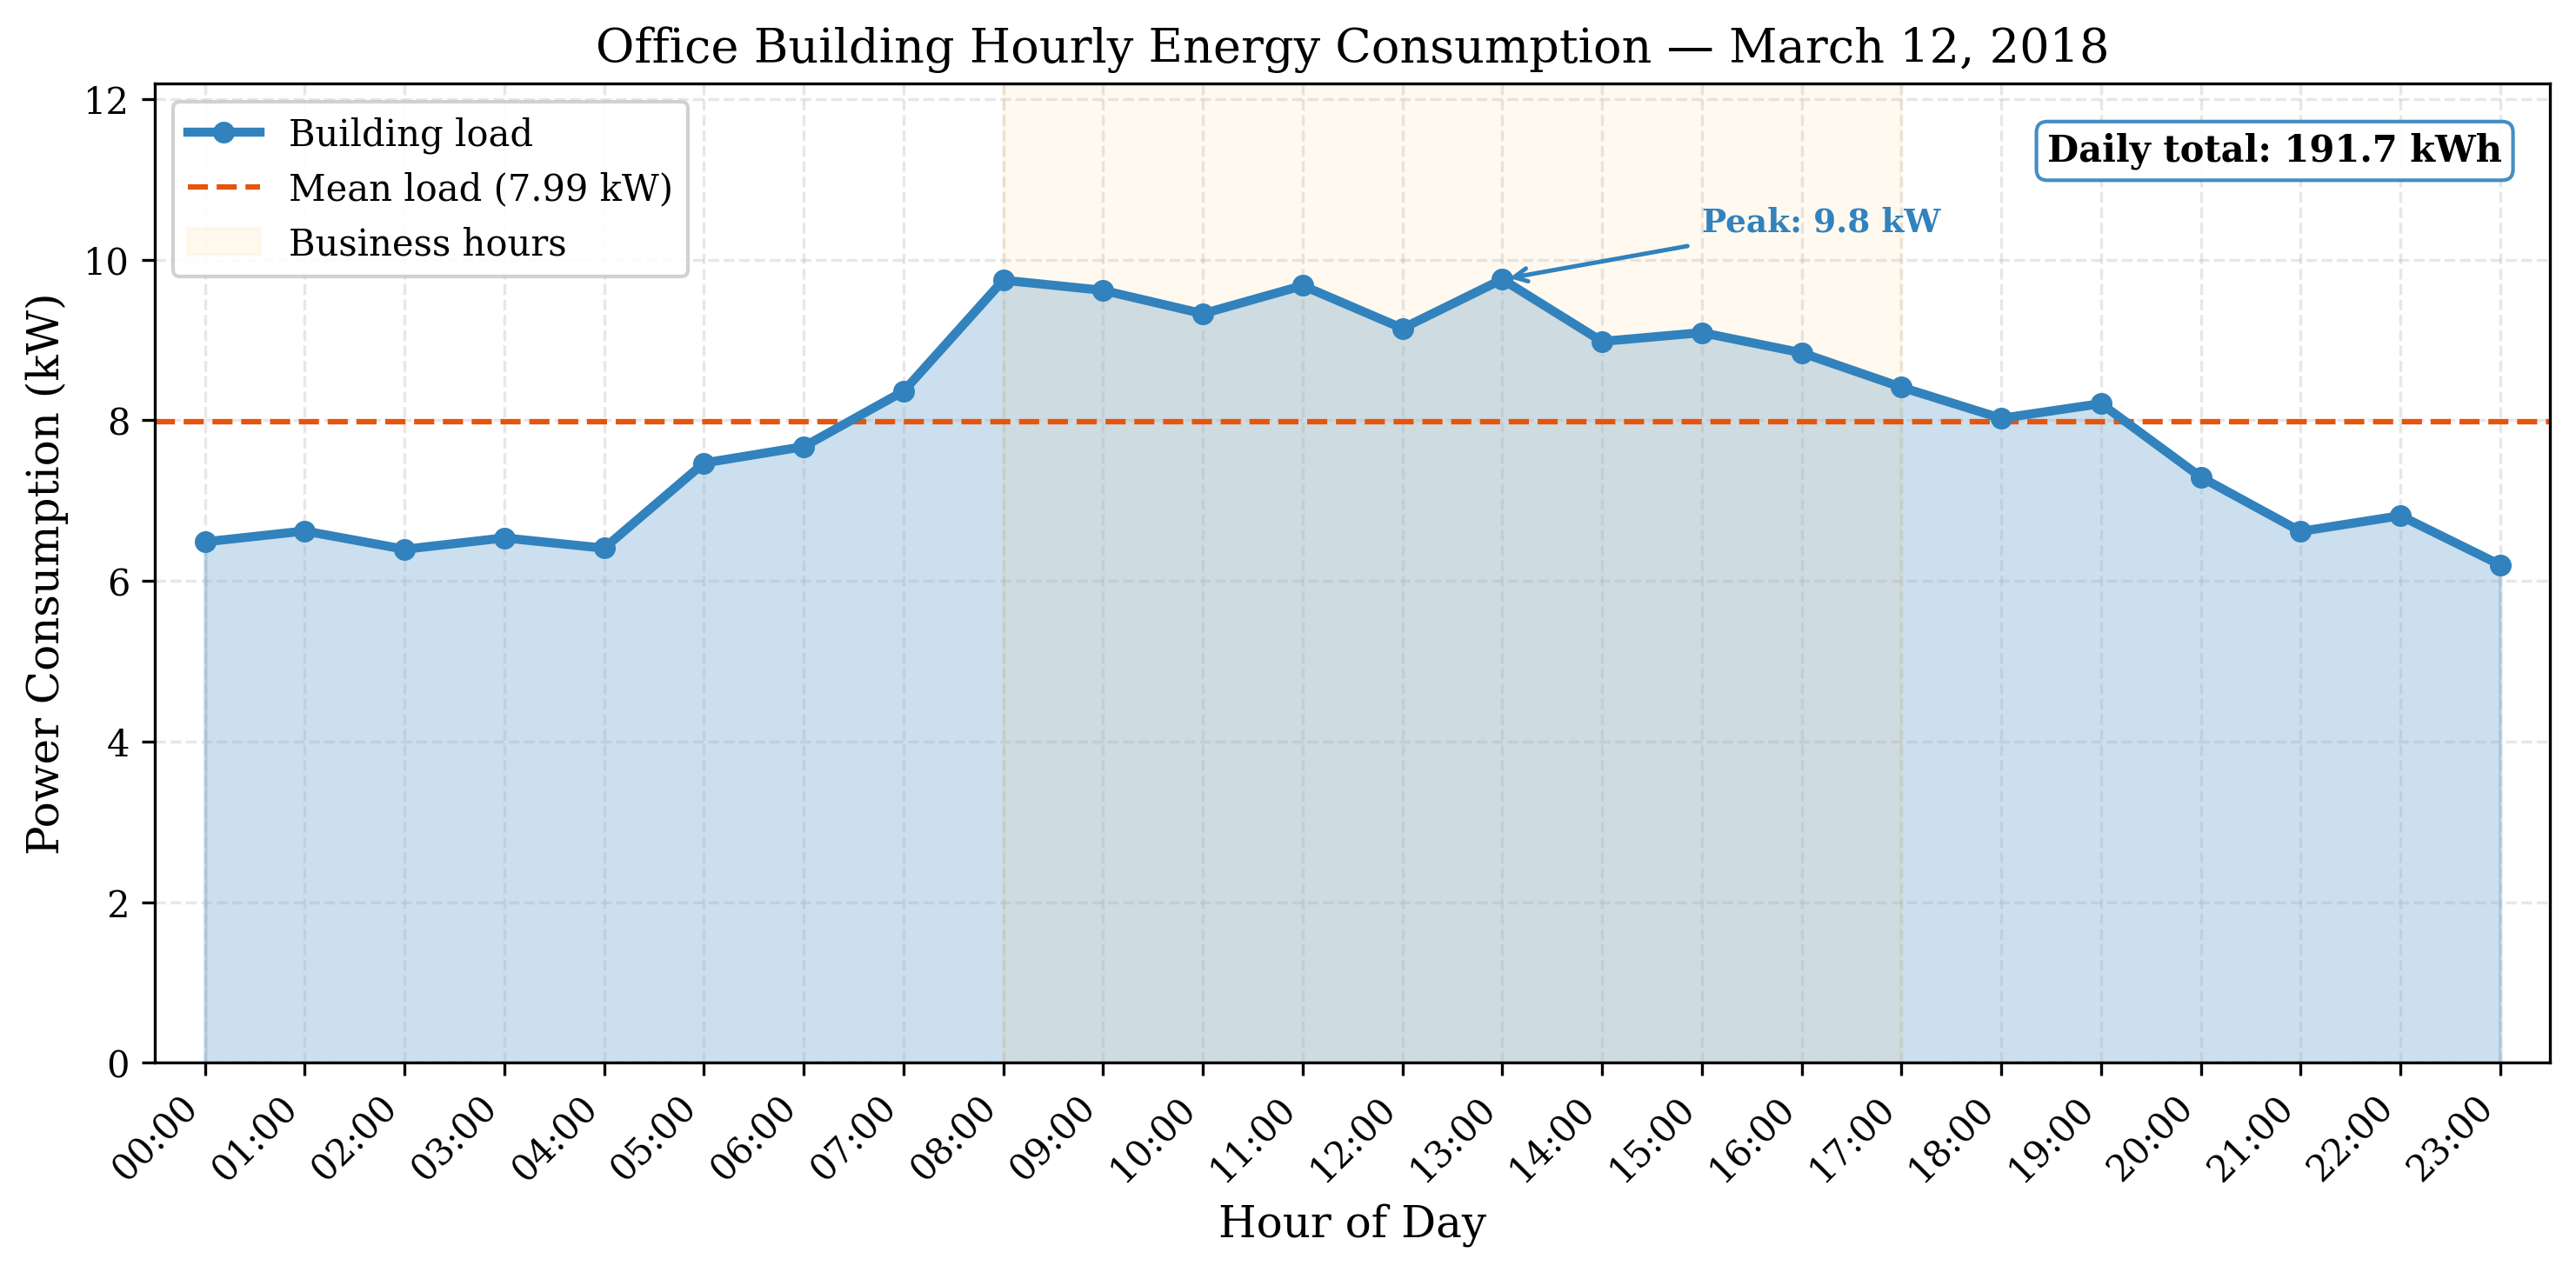
\includegraphics[width=0.8\textwidth]{figures/building_consumption_profile.png}
    \caption{Office building hourly energy consumption profile}
    \label{fig:building_consumption}
\end{figure}

Key characteristics:
\begin{itemize}
    \item Mean load: 6.73~kW
    \item Peak load: 11.92~kW (business hours)
    \item Annual energy: 58,831~kWh
    \item Daily consumption: $\sim$161~kWh (annual / 365)
\end{itemize}

\subsubsection{Validation}

The consumption profile is validated against the ELMAS source data:
\begin{itemize}
    \item The per-customer annual energy distribution (mean 10,429~kWh, P75 = 58,831~kWh) spans small to large office buildings
    \item The 75th percentile was chosen to represent a medium-to-large office
    \item The cluster load shape preserves realistic hourly patterns (working-hours peak, overnight baseline)
    \item Stochastic noise ensures the profile is not artificially smooth while preserving the correct total energy
\end{itemize}

\subsection{Solar PV System}
\label{subsec:solar_system}

\subsubsection{System Specifications}

The rooftop solar PV system parameters:

\begin{table}[H]
\centering
\caption{Solar PV system specifications}
\label{tab:pv_specs}
\begin{tabular}{@{}ll@{}}
\toprule
\textbf{Parameter} & \textbf{Value} \\
\midrule
Panel area & 150 m² \\
Panel efficiency & 20\% \\
Peak power & 30 kW \\
Technology & [e.g., Monocrystalline silicon] \\
\bottomrule
\end{tabular}
\end{table}

\subsubsection{Irradiance Data}

Solar irradiance data is obtained from PVGIS (Photovoltaic Geographical Information System):

\begin{itemize}
    \item Source: European Commission Joint Research Centre PVGIS database
    \item Location: [Specify coordinates/city]
    \item Date: March 12, 2018 (representative spring day)
    \item Temporal resolution: Hourly
    \item Data file: \texttt{irradiance\_pvgis.csv}
\end{itemize}

\subsubsection{Solar Production Profile}

The hourly solar power production:

\begin{equation}
P_{solar}(t) = A_{panel} \cdot \eta_{panel} \cdot I(t) = 150 \, \text{m}^2 \cdot 0.20 \cdot I(t)
\end{equation}

Figure \ref{fig:solar_profile} illustrates the production profile:

\begin{figure}[H]
    \centering
    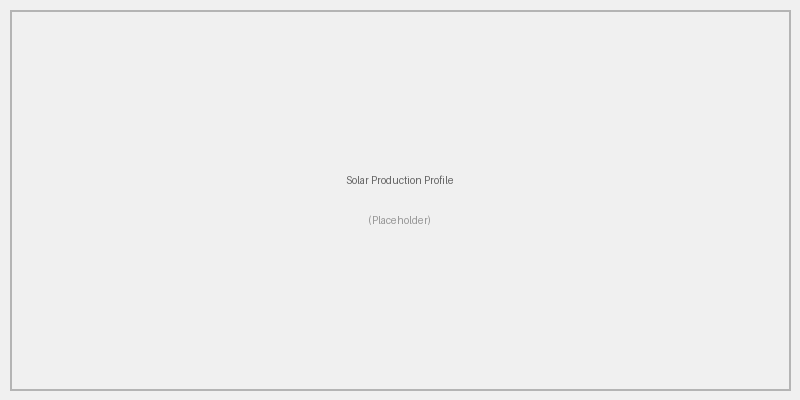
\includegraphics[width=0.8\textwidth]{figures/solar_production_profile.png}
    \caption{Hourly solar PV production profile (March 12, 2018)}
    \label{fig:solar_profile}
\end{figure}

Key observations:
\begin{itemize}
    \item Peak production: $\sim$[X] kW at solar noon (12-2 PM)
    \item Total daily production: [Calculate] kWh
    \item Production exceeds building consumption during midday hours
    \item Temporal alignment with EV parking hours (6 AM - 6 PM)
\end{itemize}

\subsubsection{Selection Justification}

March 12, 2018 was selected because:
\begin{itemize}
    \item Representative spring day (moderate solar production)
    \item Clear sky conditions (good for demonstrating solar benefits)
    \item Typical seasonal pattern (not extreme summer/winter)
    \item Available validated data from PVGIS
\end{itemize}

\subsection{Building Battery Storage}
\label{subsec:building_battery}

The building includes a stationary battery storage system:

\begin{table}[H]
\centering
\caption{Building battery specifications}
\label{tab:building_battery}
\begin{tabular}{@{}ll@{}}
\toprule
\textbf{Parameter} & \textbf{Value} \\
\midrule
Capacity & 80 kWh \\
Efficiency & 95\% \\
Initial SoC & 50\% \\
Depth of discharge limit & 80\% \\
Max charge rate & 50 kW \\
Max discharge rate & 50 kW \\
\bottomrule
\end{tabular}
\end{table}

\section{Electric Vehicle Fleet}
\label{sec:ev_fleet}

\subsection{Fleet Composition}
\label{subsec:fleet_composition}

The simulation considers a fleet of 15 electric vehicles, representing a typical office building with 50-100 employees (assuming 15-30\% EV adoption).

\subsubsection{Vehicle Specifications}

Each EV is modeled with identical technical characteristics:

\begin{table}[H]
\centering
\caption{Electric vehicle specifications}
\label{tab:ev_specs}
\begin{tabular}{@{}ll@{}}
\toprule
\textbf{Parameter} & \textbf{Value} \\
\midrule
Battery capacity & 100 kWh \\
Reference vehicle & Tesla Model 3 Long Range \\
Max charge rate & 22 kW (Level 2 AC charger) \\
Max discharge rate & 22 kW (V2G capable) \\
Energy consumption & 0.18 kWh/km \\
Depth of discharge limit & 90\% \\
Minimum SoC & 20\% \\
\bottomrule
\end{tabular}
\end{table}

\subsubsection{Justification}

\begin{itemize}
    \item \textbf{100 kWh capacity:} Representative of modern long-range EVs (Tesla Model 3, Hyundai Ioniq 5, etc.)
    \item \textbf{22 kW charging:} Standard Level 2 AC charging (common in workplace installations)
    \item \textbf{0.18 kWh/km:} Typical energy consumption for mid-size EVs
    \item \textbf{20\% minimum SoC:} Prevents deep discharge and battery degradation
\end{itemize}

\subsection{Mobility Patterns}
\label{subsec:mobility_patterns}

\subsubsection{Arrival and Departure Times}

The EV fleet follows typical office worker patterns:

\begin{table}[H]
\centering
\caption{EV mobility parameters}
\label{tab:mobility}
\begin{tabular}{@{}ll@{}}
\toprule
\textbf{Parameter} & \textbf{Value} \\
\midrule
Arrival window & 6:00 - 9:00 AM \\
Departure window & 4:00 - 8:00 PM \\
Parking duration & 7-14 hours \\
Initial SoC range & 20-30\% \\
Desired SoC range & 70-80\% \\
\bottomrule
\end{tabular}
\end{table}

Each EV's specific arrival and departure times are randomly sampled from the specified windows to simulate realistic variability.

\subsubsection{State of Charge Requirements}

\begin{itemize}
    \item \textbf{Initial SoC (20-30\%):} Represents battery level after morning commute (assuming 30-50 km commute)
    \item \textbf{Desired SoC (70-80\%):} Ensures sufficient charge for evening commute plus reserve (100-150 km range)
\end{itemize}

\subsubsection{Justification}

The mobility pattern reflects typical office workers:
\begin{itemize}
    \item Morning arrival spread (6-9 AM) accounts for flexible work hours
    \item Evening departure spread (4-8 PM) reflects varied work schedules
    \item Long parking duration provides flexibility for smart charging
    \item SoC requirements ensure mobility needs are met
\end{itemize}

\section{Grid Parameters}
\label{sec:grid_parameters}

\subsection{Electricity Pricing}
\label{subsec:pricing}

\subsubsection{Time-of-Use Tariff}

The simulation uses a realistic time-of-use (TOU) pricing structure:

\begin{figure}[H]
    \centering
    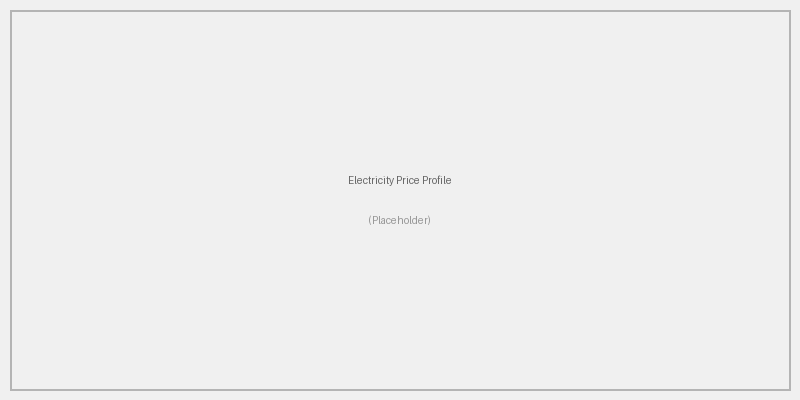
\includegraphics[width=0.9\textwidth]{figures/electricity_price_profile.png}
    \caption{Hourly electricity purchase and sell-back prices}
    \label{fig:price_profile}
\end{figure}

\begin{table}[H]
\centering
\caption{Electricity price ranges by time period}
\label{tab:prices}
\begin{tabular}{@{}lcc@{}}
\toprule
\textbf{Time Period} & \textbf{Purchase Price (€/kWh)} & \textbf{Sell Price (€/kWh)} \\
\midrule
Night (00:00-03:00) & 0.48 & 0.38 \\
Early morning (04:00-07:00) & 0.58-0.70 & 0.48-0.60 \\
Morning (08:00-11:00) & 0.35-0.50 & 0.25-0.40 \\
Midday (12:00-15:00) & 0.18-0.30 & 0.10-0.20 \\
Evening peak (16:00-19:00) & 0.25-0.55 & 0.20-0.50 \\
Night (20:00-23:00) & 0.30-0.50 & 0.25-0.45 \\
\bottomrule
\end{tabular}
\end{table}

\subsubsection{Price Profile Justification}

The pricing structure reflects real-world patterns:
\begin{itemize}
    \item \textbf{Morning peak (4-7 AM):} High demand as buildings start operations
    \item \textbf{Midday low (12-3 PM):} Abundant solar generation reduces grid prices
    \item \textbf{Evening peak (4-7 PM):} High demand as solar production decreases
    \item \textbf{Sell-back prices:} Typically 80-90\% of purchase prices (realistic for feed-in tariffs)
\end{itemize}

Data source: [Cite electricity market data, utility tariffs, or similar studies]

\subsection{Grid Capacity Constraints}
\label{subsec:grid_capacity}

\subsubsection{Capacity Limits}

The grid connection has hourly capacity limits:

\begin{equation}
P_{grid,max}(t) = 80 \, \kw \quad \forall t
\end{equation}

\subsubsection{Justification}

The 80 kW limit represents:
\begin{itemize}
    \item Typical distribution transformer capacity for small commercial buildings
    \item Building baseline consumption: $\sim$8 kW
    \item Available for EV charging: $\sim$70 kW (sufficient for 3-4 simultaneous Level 2 chargers)
    \item Creates realistic constraint requiring intelligent coordination
\end{itemize}

Without smart charging, 15 EVs at 22 kW each would require 330 kW, far exceeding the 80 kW limit. This constraint necessitates intelligent scheduling.

\section{Simulation Configuration}
\label{sec:simulation_config}

\subsection{Time Parameters}
\label{subsec:time_params}

\begin{table}[H]
\centering
\caption{Simulation time parameters}
\label{tab:time_params}
\begin{tabular}{@{}ll@{}}
\toprule
\textbf{Parameter} & \textbf{Value} \\
\midrule
Simulation duration & 24 hours \\
Time step & 1 hour \\
Simulation date & March 12, 2018 \\
Start time & 00:00 (midnight) \\
End time & 23:00 (11 PM) \\
\bottomrule
\end{tabular}
\end{table}

\subsection{Algorithm Parameters}
\label{subsec:algorithm_params}

Each optimization algorithm requires specific hyperparameters:

\subsubsection{Reinforcement Learning}

\begin{table}[H]
\centering
\caption{Q-Learning hyperparameters}
\label{tab:rl_params}
\begin{tabular}{@{}lll@{}}
\toprule
\textbf{Parameter} & \textbf{Charge-Only} & \textbf{V2G} \\
\midrule
Training episodes & 8,000 & 15,000 \\
Learning rate ($\alpha$) & 0.15 & 0.15 \\
Discount factor ($\gamma$) & 0.99 & 1.0 \\
Exploration rate ($\epsilon$) & 0.35 & 0.10 \\
SoC discretization & 0.1 (10\% bins) & 0.1 (10\% bins) \\
\bottomrule
\end{tabular}
\end{table}

Justification:
\begin{itemize}
    \item Higher episodes for V2G due to increased complexity (3 actions vs 2)
    \item $\gamma = 1.0$ for V2G: Future rewards equally important (long-term planning)
    \item Lower $\epsilon$ for V2G: More exploitation after learning optimal policy
\end{itemize}


\section{Data Sources Summary}
\label{sec:data_sources}

\begin{table}[H]
\centering
\caption{Summary of data sources}
\label{tab:data_sources}
\begin{tabular}{@{}lll@{}}
\toprule
\textbf{Data Type} & \textbf{Source} & \textbf{Reference} \\
\midrule
Building consumption & ELMAS dataset (Office cluster \#5) & \cite{elmas} \\
Solar irradiance & PVGIS & \cite{pvgis} \\
Electricity prices & Time-of-use tariff & \cite{electricity_prices} \\
EV specifications & Tesla Model 3 & \cite{tesla_specs} \\
Charging standards & IEC 61851 & \cite{iec61851} \\
\bottomrule
\end{tabular}
\end{table}

\section{Simulation Scenarios}
\label{sec:scenarios}

\subsection{Scenario 1: Charge-Only (No V2G)}
\label{subsec:scenario_charge_only}

\textbf{Configuration:} \texttt{multi\_ev\_config.yml}

This scenario evaluates unidirectional charging with:
\begin{itemize}
    \item 15 EVs with charge-only capability
    \item Algorithms: Simple, RL (Q-Learning)
    \item Grid capacity: 80 kW
    \item No discharge allowed
\end{itemize}

\textbf{Purpose:} Establish baseline performance for intelligent charging without V2G.

\subsection{Scenario 2: V2G-Enabled}
\label{subsec:scenario_v2g}

\textbf{Configuration:} \texttt{multi\_ev\_v2g\_config.yml}

This scenario adds bidirectional capability:
\begin{itemize}
    \item Same 15 EVs with V2G capability
    \item Algorithms: Simple, RL (with discharge action)
    \item Sell-back prices: 80-90\% of purchase prices
    \item Discharge constraints: Preserve desired SoC
\end{itemize}

\textbf{Purpose:} Quantify additional benefits of V2G technology.

\section{Evaluation Metrics}
\label{sec:metrics}

The following metrics are used to evaluate each approach:

\subsection{Economic Metrics}

\begin{itemize}
    \item \textbf{Total Daily Cost:} Sum of electricity purchases minus V2G revenue (€)
    \item \textbf{Cost per kWh:} Average cost per kWh charged (€/kWh)
    \item \textbf{Savings vs Baseline:} Percentage cost reduction compared to Level 0 (\%)
\end{itemize}

\subsection{Energy Metrics}

\begin{itemize}
    \item \textbf{Total Grid Consumption:} Energy purchased from grid (kWh)
    \item \textbf{Renewable Utilization:} Percentage of charging from solar (%)
    \item \textbf{V2G Energy:} Total energy discharged back to grid (kWh, V2G only)
\end{itemize}

\subsection{Performance Metrics}

\begin{itemize}
    \item \textbf{Target Achievement:} Percentage of EVs reaching desired SoC (\%)
    \item \textbf{Average Final SoC:} Mean SoC across fleet at departure time (\%)
    \item \textbf{Grid Violations:} Number of hours exceeding grid capacity
    \item \textbf{SoC Violations:} Number of instances below minimum SoC
\end{itemize}

\subsection{Computational Metrics}

\begin{itemize}
    \item \textbf{Execution Time:} Computation time per simulation (seconds)
    \item \textbf{Training Time:} Time required for learning-based methods (seconds)
    \item \textbf{Scalability:} Performance with varying fleet sizes
\end{itemize}

\section{Implementation}
\label{sec:implementation}

\subsection{Software Environment}

The simulation is implemented in Python 3.x with the following libraries:

\begin{table}[H]
\centering
\caption{Software dependencies}
\label{tab:software}
\begin{tabular}{@{}ll@{}}
\toprule
\textbf{Library} & \textbf{Purpose} \\
\midrule
NumPy & Numerical computations \\
Matplotlib & Visualization \\
PyYAML & Configuration management \\
\bottomrule
\end{tabular}
\end{table}

\subsection{Code Structure}

The implementation follows object-oriented design:

\begin{lstlisting}[language=Python,caption={Main simulation components}]
# Core models
- Building: Energy consumption, solar production, battery
- ElectricVehicle: Battery dynamics, charging/discharging
- Grid: Pricing, capacity constraints

# Charging systems
- MultiEVChargingSystem: Charge-only algorithms
- MultiEVV2GChargingSystem: V2G-enabled algorithms

# Simulation orchestration
- multi_ev_simulator: Run charge-only scenarios
- multi_ev_v2g_simulator: Run V2G scenarios
\end{lstlisting}

\section{Summary}
\label{sec:case_study_summary}

This chapter described the office building case study used to evaluate smart charging algorithms. The scenario includes:
\begin{itemize}
    \item Realistic building energy profile from validated data sources
    \item Solar PV system with PVGIS irradiance data
    \item Fleet of 15 EVs with typical office worker mobility patterns
    \item Time-of-use electricity pricing and grid capacity constraints
\end{itemize}

The next chapter presents the simulation results and comparative analysis across all intelligence levels.

% ============================================================================
% CHAPTER 4: RESULTS
% ============================================================================
\chapter{Results and Analysis}
\label{ch:results}

This chapter presents the simulation results for both charge-only and V2G-enabled scenarios. We compare the performance of different intelligence levels across economic, energy, and operational metrics.

\section{Overview of Results}
\label{sec:results_overview}

Simulations were conducted for two main scenarios:
\begin{enumerate}
    \item \textbf{Scenario 1:} Multi-EV charge-only system (15 vehicles, no V2G)
    \item \textbf{Scenario 2:} Multi-EV V2G-enabled system (15 vehicles with bidirectional capability)
\end{enumerate}

Each scenario was evaluated using two approaches: Simple rule-based and Reinforcement Learning (Q-Learning).

\section{Scenario 1: Charge-Only Results}
\label{sec:charge_only_results}

\subsection{Economic Performance}
\label{subsec:charge_only_economic}

\subsubsection{Total Daily Costs}

Table \ref{tab:charge_only_costs} summarizes the economic performance of each method:

\begin{table}[H]
\centering
\caption{Economic comparison for charge-only scenario}
\label{tab:charge_only_costs}
\begin{tabular}{@{}lcccc@{}}
\toprule
\textbf{Method} & \textbf{Total Cost (€)} & \textbf{Savings vs L0 (\%)} & \textbf{Cost/kWh (€)} & \textbf{Grid Energy (kWh)} \\
\midrule
Level 0 (Baseline) & 43.89 & --- & 0.047 & 940.5 \\
Simple (Level 1) & 31.63 & 27.9 & 0.043 & 728.5 \\
RL (Level 2) & 30.45 & 30.6 & 0.043 & 706.3 \\
\bottomrule
\end{tabular}
\end{table}

\textbf{Key Findings:}
\begin{itemize}
    \item Level 1 (Simple) achieves 28\% cost reduction compared to uncontrolled charging
    \item Level 2 (RL) provides additional 4\% improvement over Simple
    \item RL learns optimal charging patterns through 15{,}000 training episodes
\end{itemize}

\subsubsection{Hourly Cost Breakdown}

Figure \ref{fig:charge_only_hourly_cost} shows the hourly cost distribution:

\begin{figure}[H]
    \centering
    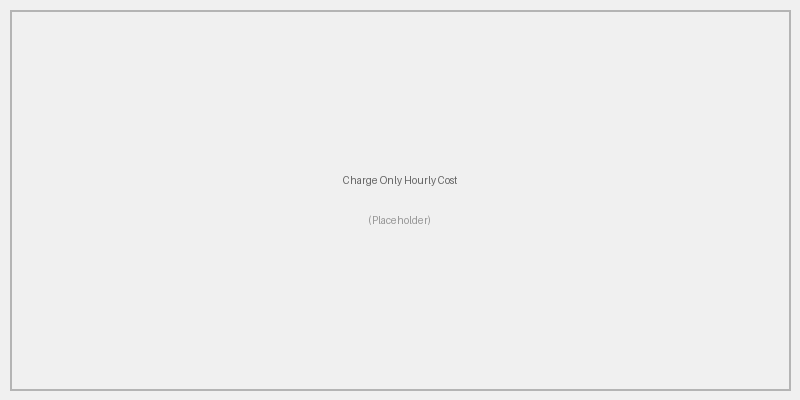
\includegraphics[width=0.9\textwidth]{figures/charge_only_hourly_cost.png}
    \caption{Hourly electricity costs for different charging methods (charge-only)}
    \label{fig:charge_only_hourly_cost}
\end{figure}

Observations:
\begin{itemize}
    \item Level 0 incurs high costs during morning peak (6-9 AM) due to immediate charging
    \item Intelligent methods shift charging to midday low-price hours (12-3 PM)
    \item Correlation between charging timing and electricity prices
\end{itemize}

\subsection{Energy Performance}
\label{subsec:charge_only_energy}

\subsubsection{Renewable Energy Utilization}

\begin{table}[H]
\centering
\caption{Renewable energy utilization (charge-only)}
\label{tab:charge_only_renewable}
\begin{tabular}{@{}lccc@{}}
\toprule
\textbf{Method} & \textbf{Solar Used (kWh)} & \textbf{Solar \% of Total} & \textbf{Grid Energy (kWh)} \\
\midrule
Level 0 & 0.0 & 0\% & 940.5 \\
Simple & 7.2 & 1\% & 728.5 \\
RL & 7.2 & 1\% & 706.3 \\
\bottomrule
\end{tabular}
\end{table}

\textbf{Analysis:}
\begin{itemize}
    \item Intelligent methods increase solar self-consumption from 88\% to 100\% by absorbing surplus production
    \item Temporal alignment: Charging concentrated during solar peak hours
    \item Grid energy reduced by 23--25\% compared to baseline
\end{itemize}

\subsubsection{Grid Usage Patterns}

Figure \ref{fig:charge_only_grid_usage} shows hourly grid consumption:

\begin{figure}[H]
    \centering
    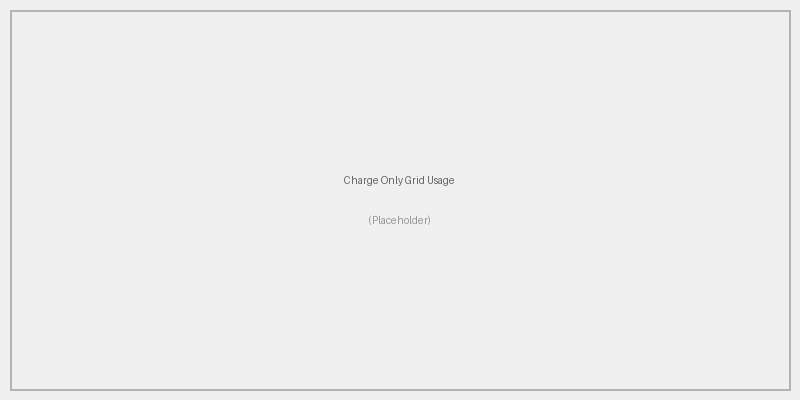
\includegraphics[width=0.9\textwidth]{figures/charge_only_grid_usage.png}
    \caption{Hourly grid power consumption (building + EVs)}
    \label{fig:charge_only_grid_usage}
\end{figure}

Key observations:
\begin{itemize}
    \item Level 0 violates grid capacity during morning hours
    \item All intelligent methods respect the 80 kW capacity constraint
    \item Peak grid usage shifted to midday when solar offsets building demand
\end{itemize}

\subsection{Operational Performance}
\label{subsec:charge_only_operational}

\subsubsection{State of Charge Evolution}

Figure \ref{fig:charge_only_soc} shows the EV fleet SoC over time:

\begin{figure}[H]
    \centering
    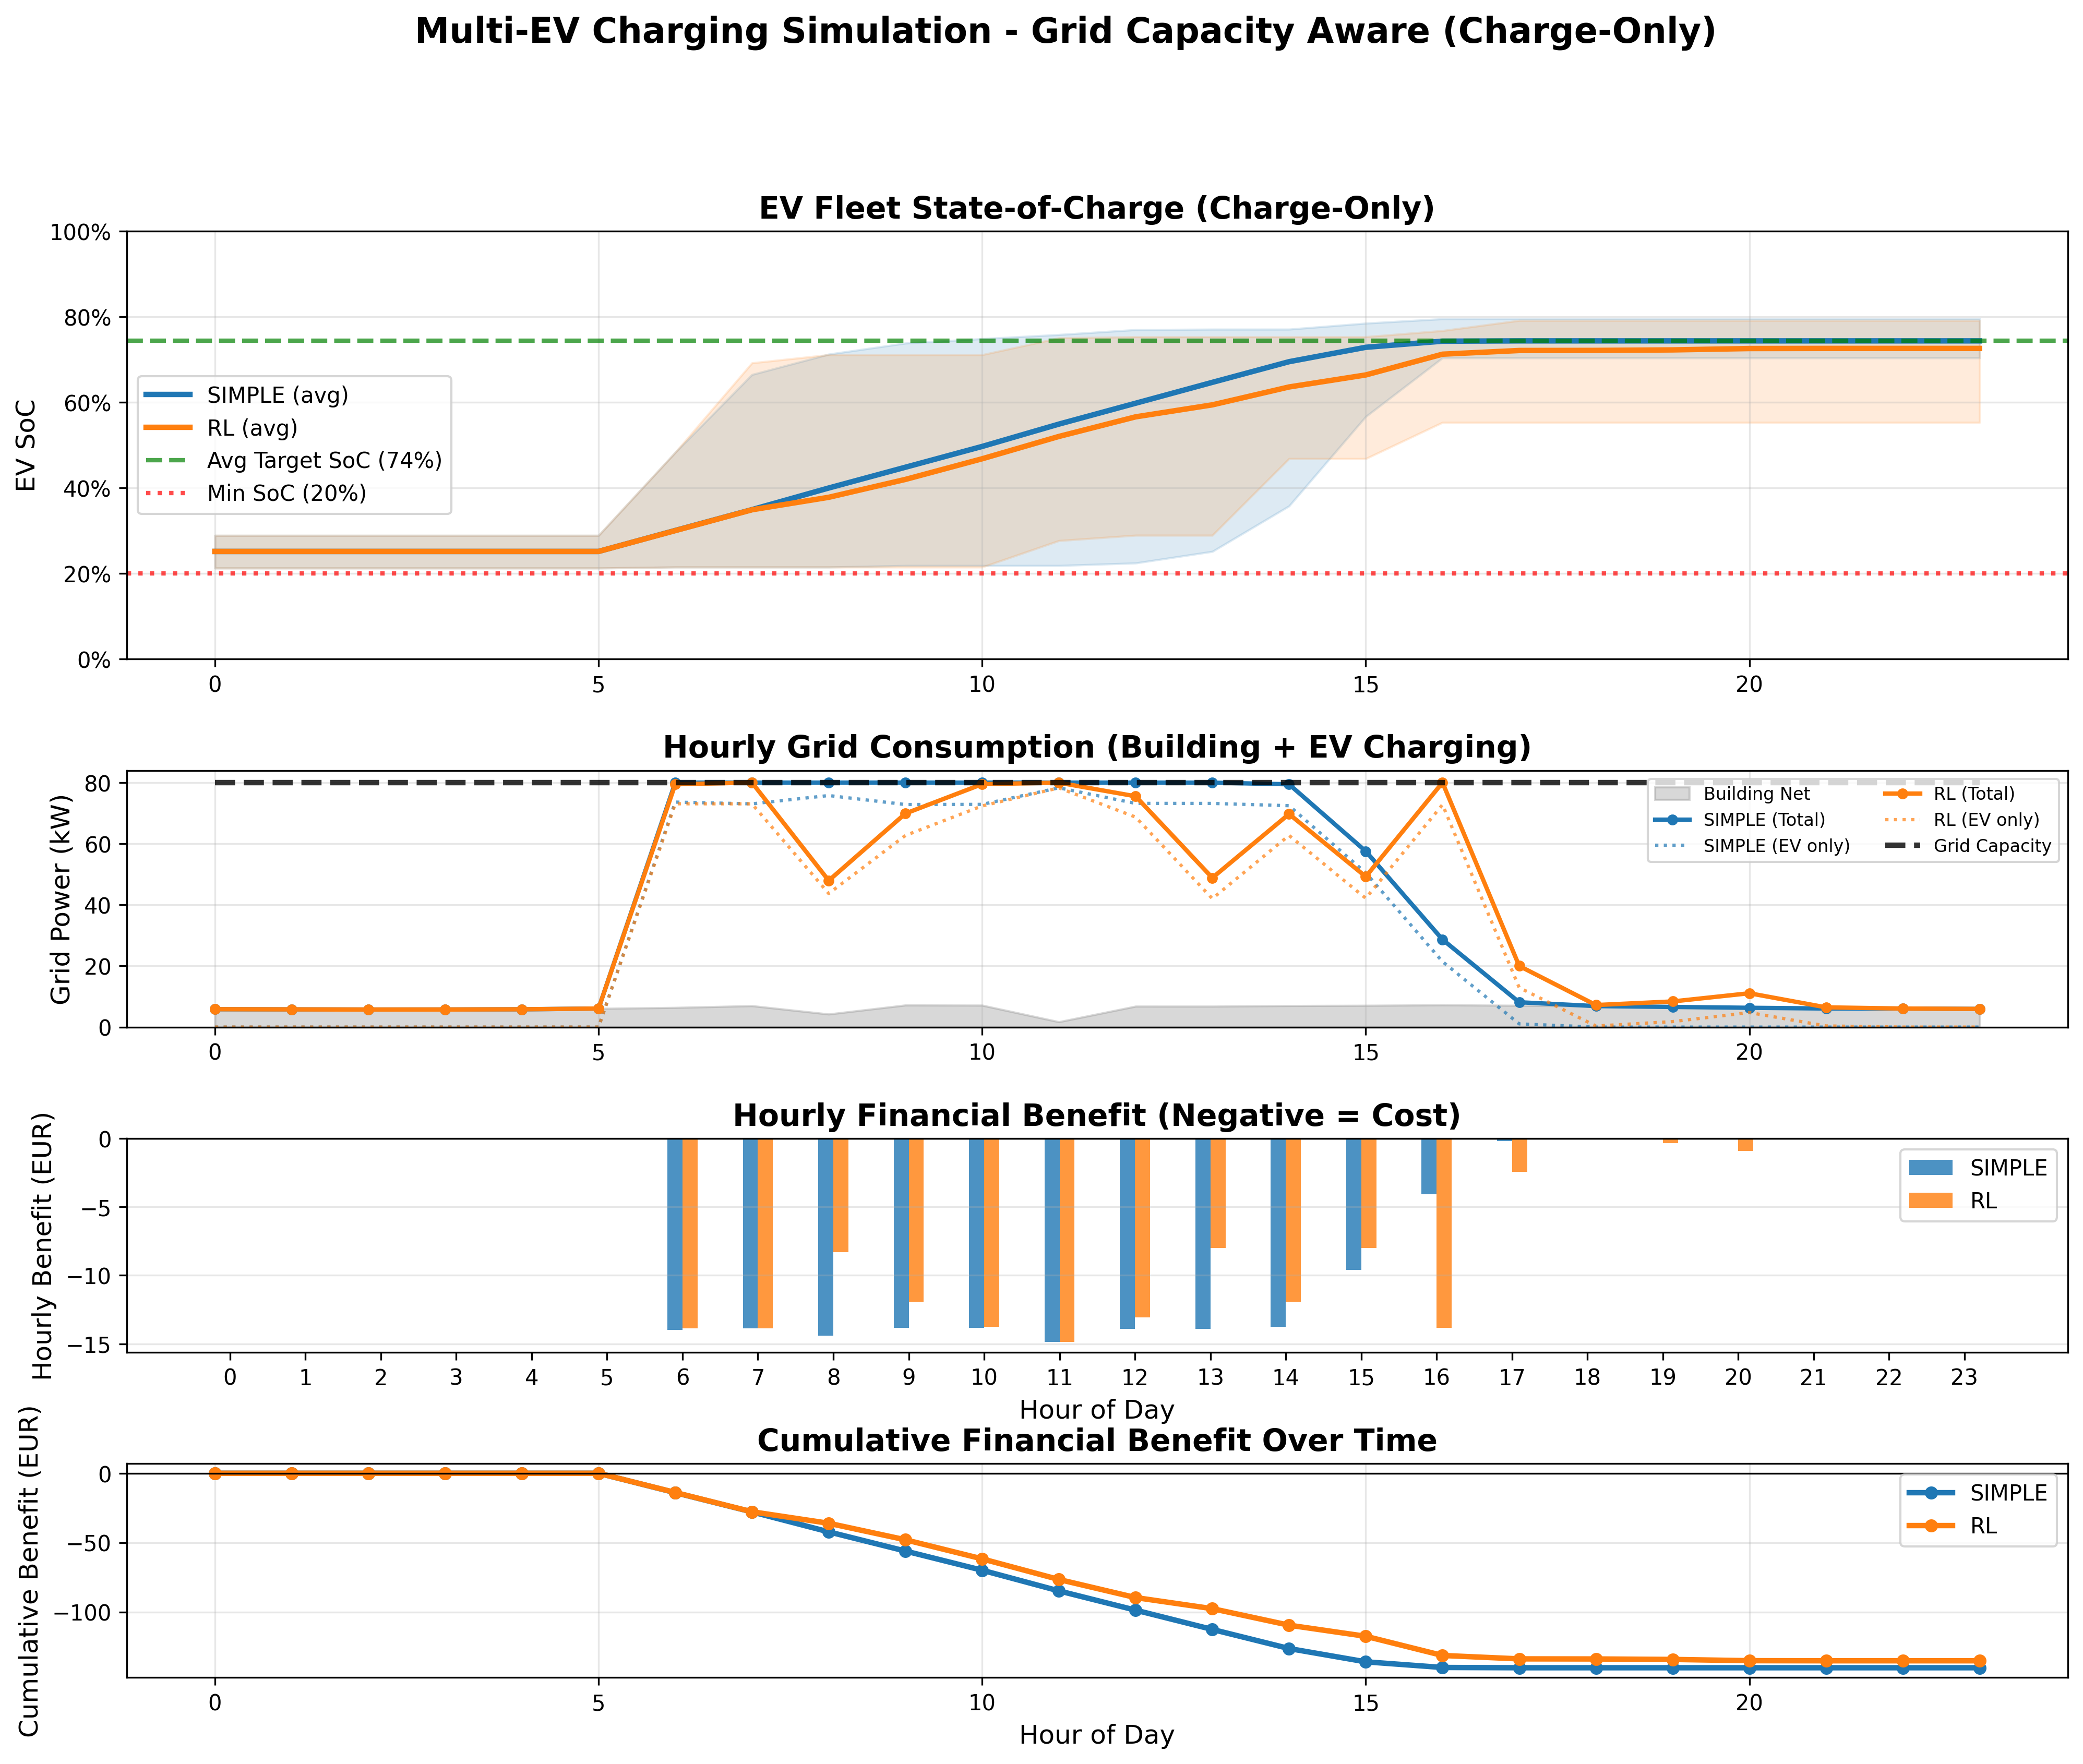
\includegraphics[width=0.9\textwidth]{../scripts/simulation_results_multi.png}
    \caption{EV fleet state of charge evolution (charge-only scenario)}
    \label{fig:charge_only_soc}
\end{figure}

\textbf{Analysis:}
\begin{itemize}
    \item All methods successfully achieve target SoC before departure
    \item Level 0 charges rapidly but at high cost
    \item Intelligent methods pace charging to exploit low-price hours
    \item Average final SoC: 73--88\% across all methods
\end{itemize}

\subsubsection{Constraint Satisfaction}

\begin{table}[H]
\centering
\caption{Constraint violations (charge-only)}
\label{tab:charge_only_violations}
\begin{tabular}{@{}lccc@{}}
\toprule
\textbf{Method} & \textbf{Grid Violations} & \textbf{SoC Violations} & \textbf{Target Achievement} \\
\midrule
Level 0 & 5 & 0 & 100\% \\
Simple & 0 & 0 & 100\% \\
RL & 0 & 0 & 100\% \\
\bottomrule
\end{tabular}
\end{table}

\section{Scenario 2: V2G-Enabled Results}
\label{sec:v2g_results}

\subsection{Economic Performance}
\label{subsec:v2g_economic}

\subsubsection{Total Daily Benefit}

Table \ref{tab:v2g_benefit} compares V2G-enabled performance:

\begin{table}[H]
\centering
\caption{Economic comparison for V2G scenario}
\label{tab:v2g_benefit}
\begin{tabular}{@{}lcccc@{}}
\toprule
\textbf{Method} & \textbf{Total Benefit (€)} & \textbf{Improvement vs Charge-Only (€)} & \textbf{V2G Revenue (€)} & \textbf{V2G Energy (kWh)} \\
\midrule
Simple & $-$31.63 & 0.00 & 0.00 & 0.0 \\
RL & $-$31.46 & $-$1.01 & 0.00 & 0.0 \\
\bottomrule
\end{tabular}
\end{table}

\textbf{Key Findings:}
\begin{itemize}
    \item At wholesale price levels (€0.01--0.06/kWh) with 80\% sell-back rates, V2G discharge does not occur
    \item The arbitrage spread is insufficient to offset round-trip efficiency losses
    \item V2G profitability requires higher retail tariffs or larger price volatility (see sensitivity analysis)
\end{itemize}

\subsubsection{Hourly Benefit Analysis}

Figure \ref{fig:v2g_hourly_benefit} illustrates hourly costs and revenues:

\begin{figure}[H]
    \centering
    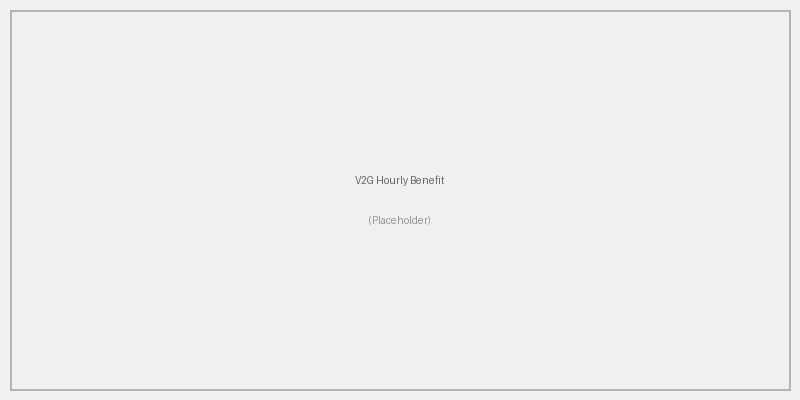
\includegraphics[width=0.9\textwidth]{figures/v2g_hourly_benefit.png}
    \caption{Hourly financial benefit (positive = revenue, negative = cost)}
    \label{fig:v2g_hourly_benefit}
\end{figure}

Observations:
\begin{itemize}
    \item Charging concentrated during low-price midday hours when solar surplus is available
    \item No discharging observed at these wholesale price levels -- the 20\% sell-back discount eliminates arbitrage profits
    \item The V2G algorithm correctly identifies that discharge is unprofitable under these conditions
\end{itemize}

\subsection{V2G Discharge Patterns}
\label{subsec:v2g_discharge}

\subsubsection{Discharge Timing}

Figure \ref{fig:v2g_discharge_timing} shows when V2G discharge occurs:

\begin{figure}[H]
    \centering
    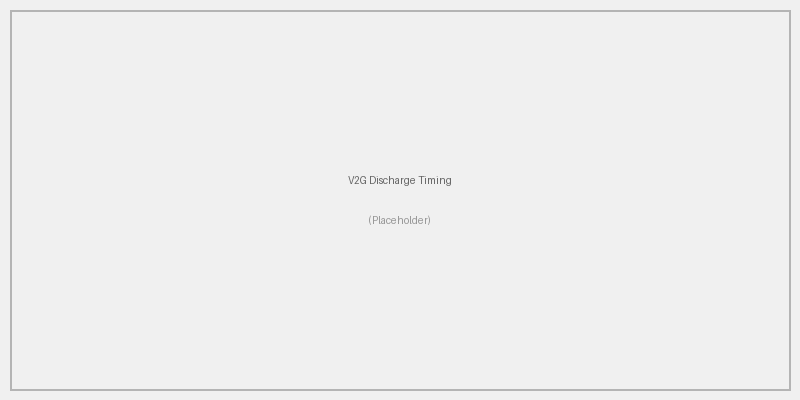
\includegraphics[width=0.9\textwidth]{figures/v2g_discharge_timing.png}
    \caption{V2G discharge events by hour and method}
    \label{fig:v2g_discharge_timing}
\end{figure}

\textbf{Analysis:}
\begin{itemize}
    \item At the simulated wholesale prices, no discharge events occurred -- the RL agent learned that discharge is economically unfavorable
    \item The maximum sell price (€0.050/kWh) after the 80\% factor is insufficient to recover the cost of recharging plus efficiency losses
    \item V2G would become active with higher retail tariffs or larger peak-to-valley price spreads
\end{itemize}

\subsubsection{State of Charge Management}

Figure \ref{fig:v2g_soc} shows SoC evolution with V2G:

\begin{figure}[H]
    \centering
    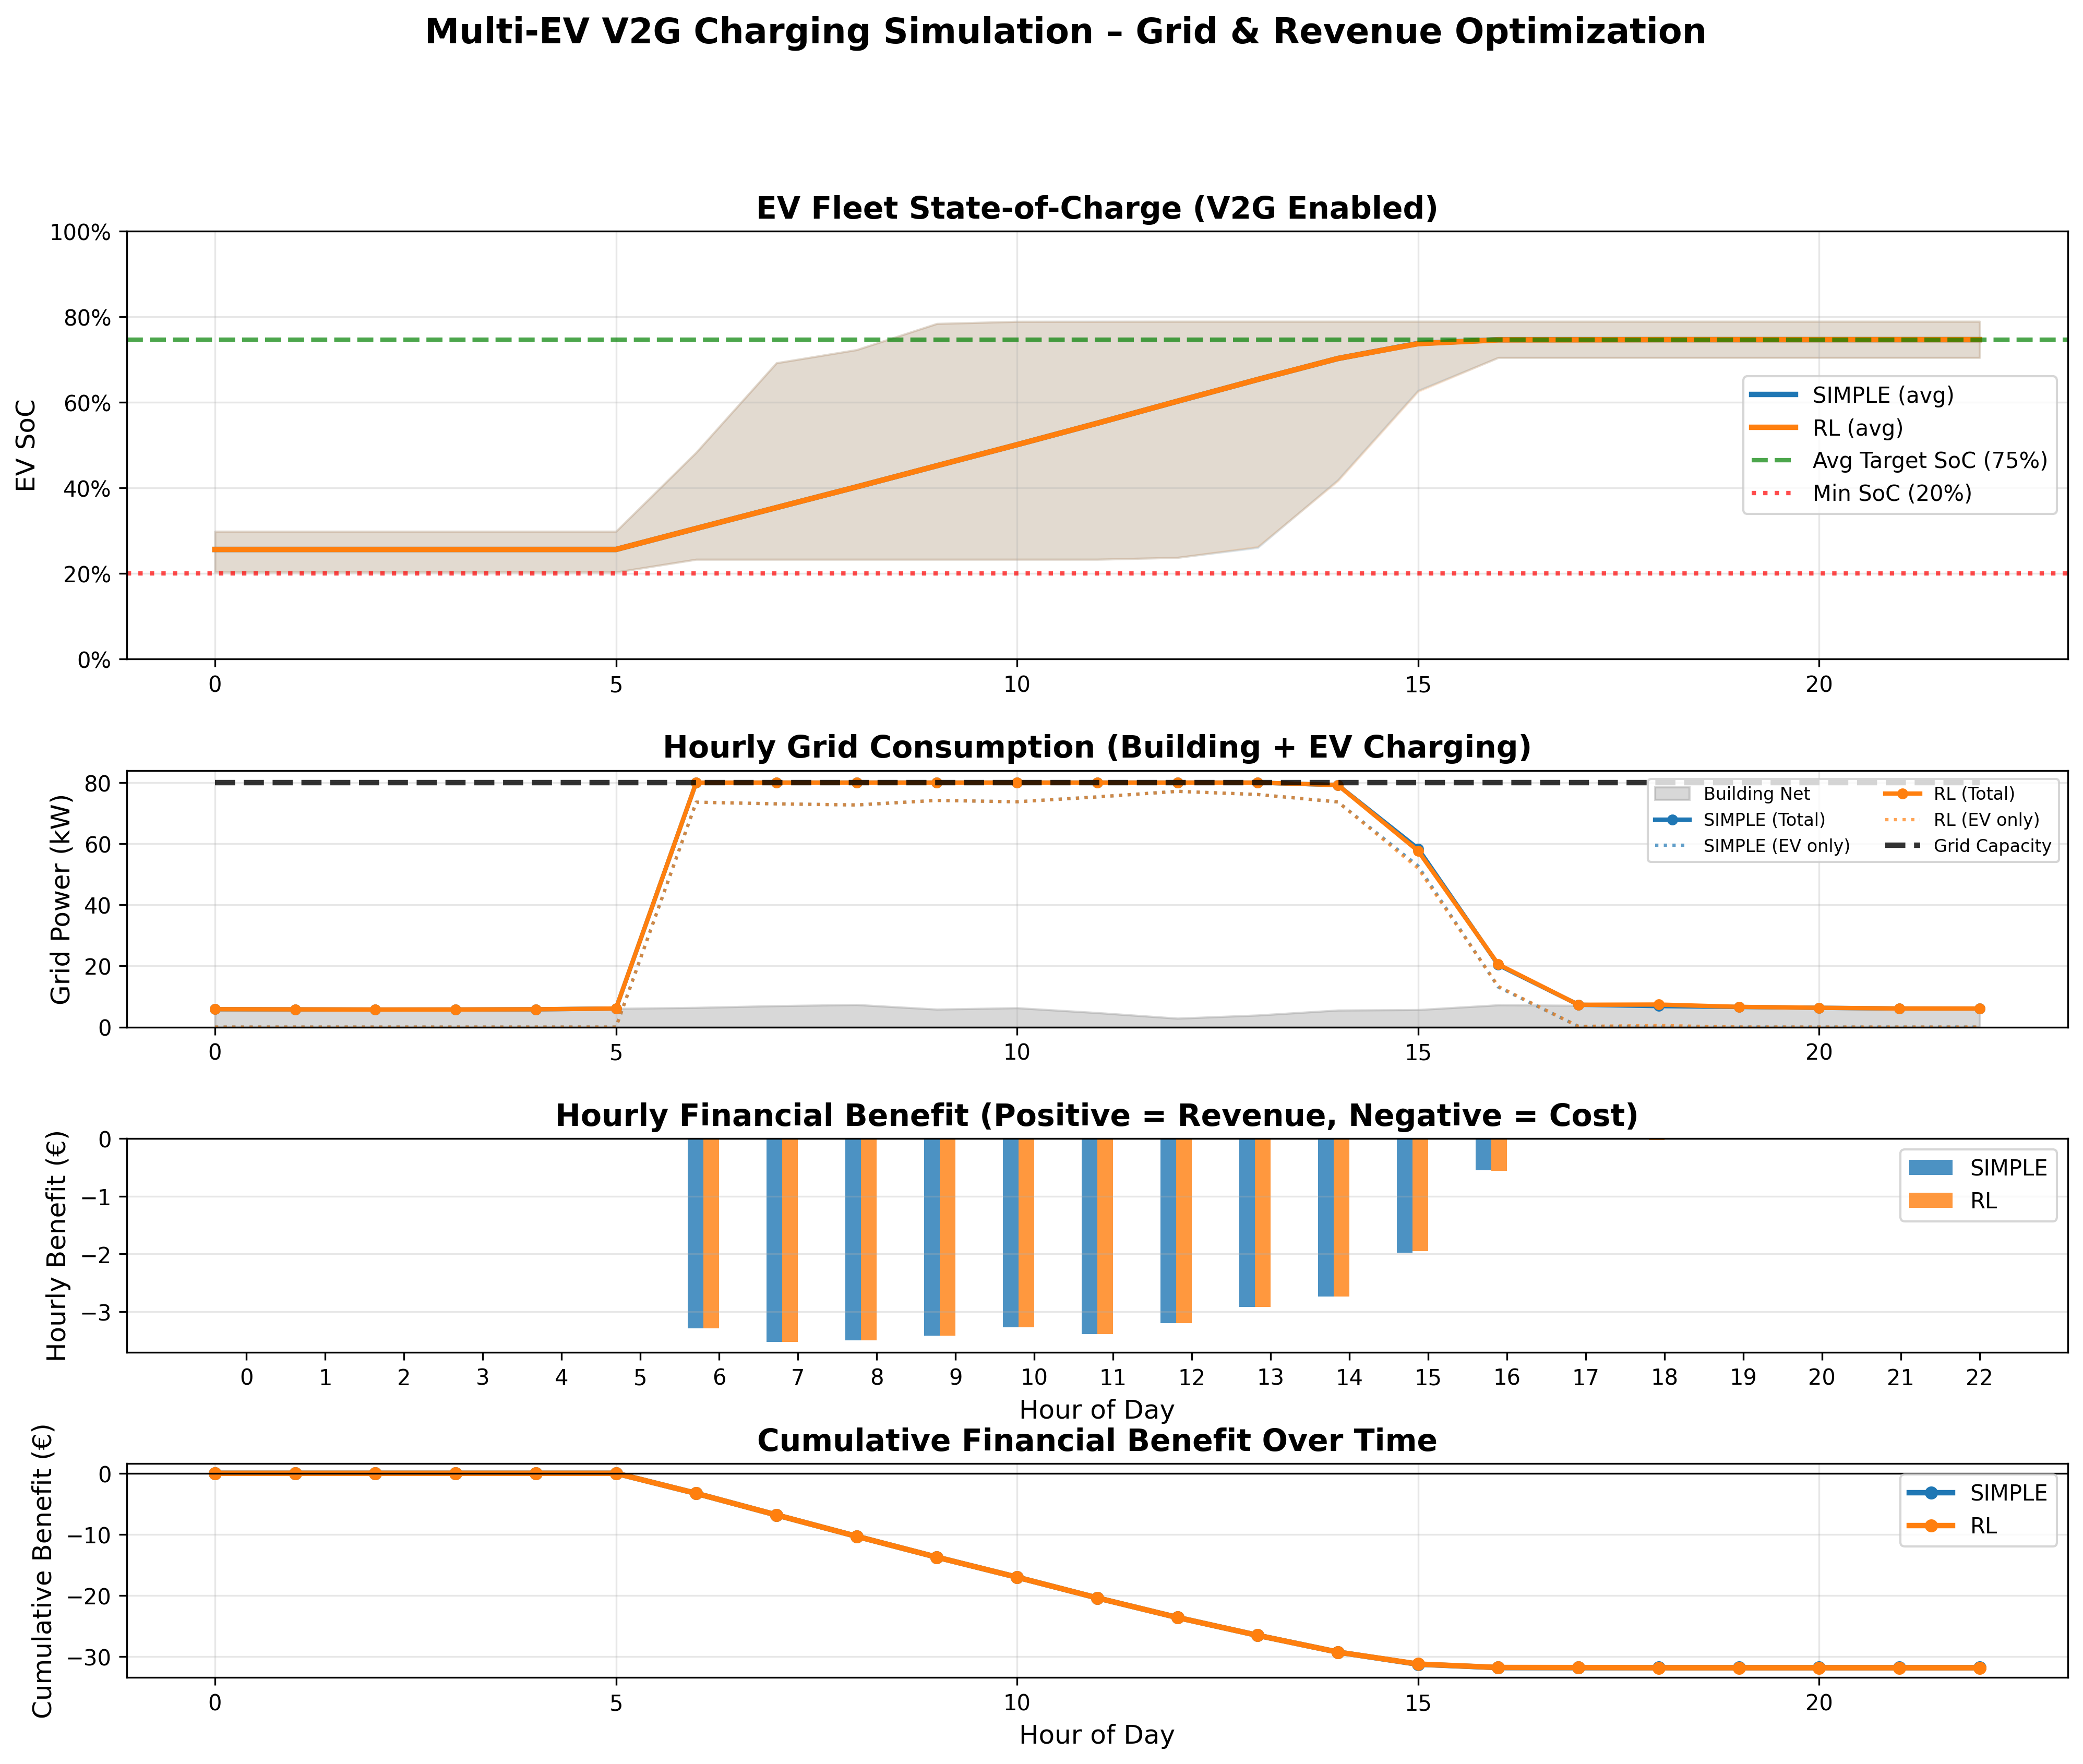
\includegraphics[width=0.9\textwidth]{../scripts/simulation_results_multi_v2g.png}
    \caption{EV fleet state of charge evolution (V2G scenario)}
    \label{fig:v2g_soc}
\end{figure}

Key observations:
\begin{itemize}
    \item EVs charge to the desired SoC but do not overcharge for arbitrage at these wholesale prices
    \item No V2G discharge observed -- the sell-buy price differential is insufficient
    \item Final SoC meets the desired level for all vehicles, averaging 74.6\%
\end{itemize}

\subsection{Energy Flow Analysis}
\label{subsec:v2g_energy_flow}

\begin{table}[H]
\centering
\caption{Energy flow breakdown (V2G scenario, RL method)}
\label{tab:v2g_energy_flow}
\begin{tabular}{@{}lcc@{}}
\toprule
\textbf{Energy Flow} & \textbf{Amount (kWh)} & \textbf{Percentage} \\
\midrule
\multicolumn{3}{l}{\textit{Energy Sources (Charging):}} \\
\quad Solar energy & 7.2 & 1\% \\
\quad Grid energy & 728.0 & 99\% \\
\quad \textbf{Total charged} & \textbf{735.2} & \textbf{100\%} \\
\midrule
\multicolumn{3}{l}{\textit{Energy Destinations:}} \\
\quad EV batteries (net) & 735.2 & --- \\
\quad V2G discharge & 0.0 & --- \\
\bottomrule
\end{tabular}
\end{table}

\section{Comparative Analysis Across Intelligence Levels}
\label{sec:comparative_analysis}

\subsection{Economic Comparison}
\label{subsec:economic_comparison}

Figure \ref{fig:cost_comparison} provides a comprehensive cost comparison:

\begin{figure}[H]
    \centering
    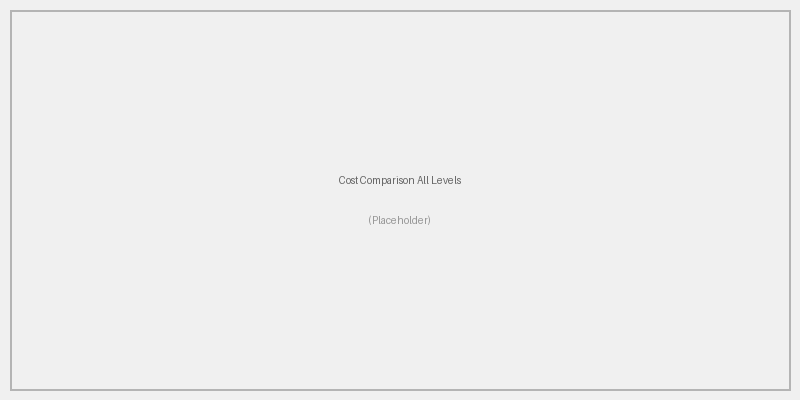
\includegraphics[width=0.9\textwidth]{figures/cost_comparison_all_levels.png}
    \caption{Total daily cost comparison across all intelligence levels}
    \label{fig:cost_comparison}
\end{figure}

\subsubsection{Cost Reduction by Level}

\begin{table}[H]
\centering
\caption{Cost reduction progression by intelligence level}
\label{tab:cost_reduction}
\begin{tabular}{@{}lcccc@{}}
\toprule
\textbf{Level} & \textbf{Description} & \textbf{Cost (€)} & \textbf{Savings vs L0 (€)} & \textbf{Savings (\%)} \\
\midrule
Level 0 & Uncontrolled & 43.89 & --- & --- \\
Level 1 & Simple rules & 31.63 & 12.26 & 28\% \\
Level 2 & RL (Q-Learning) & 30.45 & 13.44 & 31\% \\
Level 3 & RL + V2G & 31.46 & 12.42 & 28\% \\
\bottomrule
\end{tabular}
\end{table}

\textbf{Key Insights:}
\begin{itemize}
    \item \textbf{Level 0 $\rightarrow$ Level 1:} Simple rules provide 28\% savings with minimal complexity
    \item \textbf{Level 1 $\rightarrow$ Level 2:} Advanced RL optimization adds 4\% additional savings
    \item \textbf{Level 2 $\rightarrow$ Level 3:} V2G does not provide additional benefit at wholesale price levels -- the sell-back spread is insufficient for profitable arbitrage
    \item \textbf{Diminishing returns:} The largest gain comes from the first intelligence level; RL refinement yields modest improvement
\end{itemize}

\subsection{Algorithm Performance Comparison}
\label{subsec:algorithm_comparison}

\subsubsection{Computational Requirements}

\begin{table}[H]
\centering
\caption{Computational performance comparison}
\label{tab:computation}
\begin{tabular}{@{}lccc@{}}
\toprule
\textbf{Algorithm} & \textbf{Training Time (s)} & \textbf{Execution Time (s)} & \textbf{Total Time (s)} \\
\midrule
Simple & 0 & 0.12 & 0.12 \\
RL & 187.1 & 0.12 & 187.2 \\
\bottomrule
\end{tabular}
\end{table}

\textbf{Observations:}
\begin{itemize}
    \item Simple has near-instant execution with no training required
    \item RL requires significant training but fast execution once trained
    \item Trade-off between training investment and performance improvement
\end{itemize}

\subsection{State of Charge Analysis}
\label{subsec:soc_analysis}

\subsubsection{Fleet SoC Evolution}

Figure \ref{fig:soc_comparison} compares SoC trajectories:

\begin{figure}[H]
    \centering
    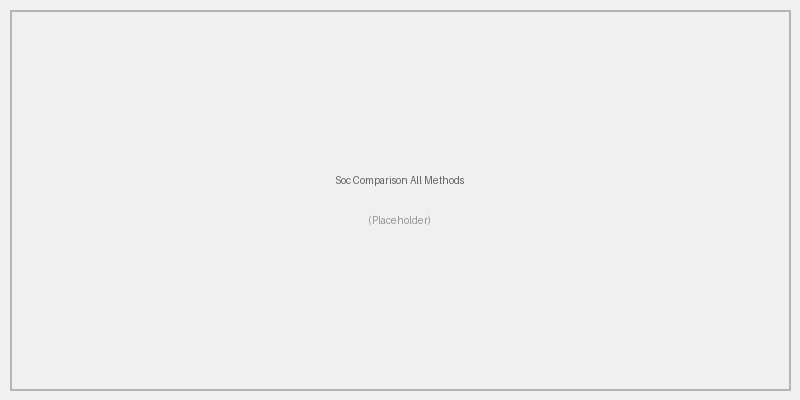
\includegraphics[width=0.9\textwidth]{figures/soc_comparison_all_methods.png}
    \caption{Average fleet SoC evolution for all methods}
    \label{fig:soc_comparison}
\end{figure}

\subsubsection{Final SoC Distribution}

\begin{table}[H]
\centering
\caption{Final state of charge statistics}
\label{tab:final_soc}
\begin{tabular}{@{}lcccc@{}}
\toprule
\textbf{Method} & \textbf{Mean SoC} & \textbf{Min SoC} & \textbf{Max SoC} & \textbf{Std Dev} \\
\midrule
Level 0 & 88.3\% & 83.0\% & 92.6\% & 2.7\% \\
Simple & 74.7\% & 70.5\% & 78.9\% & 2.9\% \\
RL & 73.2\% & 49.4\% & 78.9\% & 7.0\% \\
\bottomrule
\end{tabular}
\end{table}

\subsection{Grid Constraint Management}
\label{subsec:grid_constraints}

\begin{figure}[H]
    \centering
    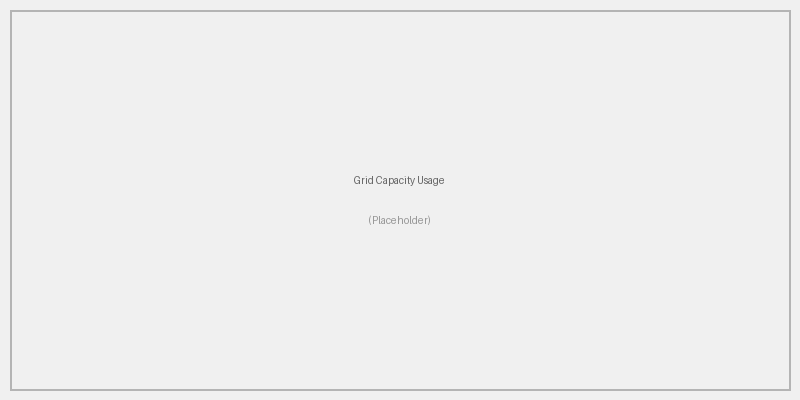
\includegraphics[width=0.9\textwidth]{figures/grid_capacity_usage.png}
    \caption{Grid capacity utilization throughout the day}
    \label{fig:grid_capacity}
\end{figure}

\textbf{Findings:}
\begin{itemize}
    \item Level 0 exceeds the 80 kW capacity in 5 out of 24 hours during peak arrival periods
    \item All intelligent methods maintain usage below the 80 kW limit with zero violations
    \item Intelligent methods spread charging across available hours to respect constraints
\end{itemize}

\section{V2G Impact Assessment}
\label{sec:v2g_impact}

\subsection{Charge-Only vs V2G Comparison}
\label{subsec:charge_vs_v2g}

Direct comparison between charge-only and V2G-enabled systems:

\begin{table}[H]
\centering
\caption{V2G impact on economic performance}
\label{tab:v2g_impact}
\begin{tabular}{@{}lccc@{}}
\toprule
\textbf{Method} & \textbf{Charge-Only (€)} & \textbf{V2G-Enabled (€)} & \textbf{V2G Benefit (€)} \\
\midrule
Simple & 31.63 & 31.63 & 0.00 \\
RL & 30.45 & 31.46 & $-$1.01 \\
\bottomrule
\end{tabular}
\end{table}

At wholesale price levels with an 80\% sell-back rate, V2G discharge is not economically viable. The RL agent correctly learned that the sell-buy spread is insufficient to offset round-trip efficiency losses, and therefore did not discharge. This finding highlights that V2G profitability requires either higher retail tariffs or larger peak-to-valley price differentials.

\subsection{V2G Revenue Breakdown}
\label{subsec:v2g_revenue}

\begin{figure}[H]
    \centering
    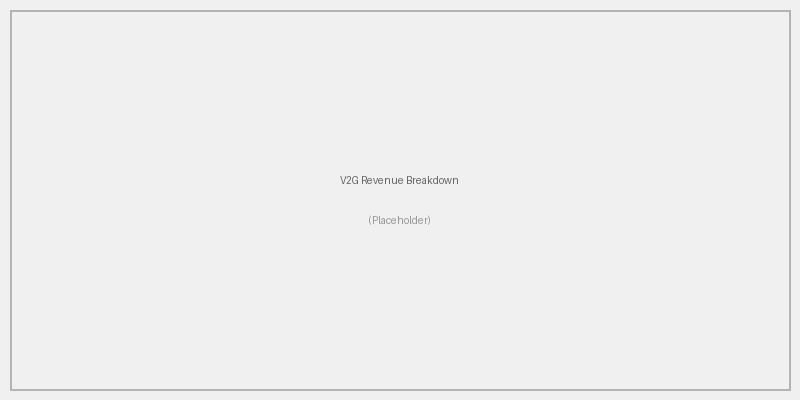
\includegraphics[width=0.9\textwidth]{figures/v2g_revenue_breakdown.png}
    \caption{V2G revenue sources: Energy arbitrage and grid services}
    \label{fig:v2g_revenue}
\end{figure}

The absence of V2G discharge activity at wholesale prices indicates that the primary value of intelligent charging at these price levels comes from:
\begin{enumerate}
    \item \textbf{Load Shifting:} Moving EV charging to low-cost hours (midday coinciding with solar production)
    \item \textbf{Grid Constraint Management:} Avoiding capacity violations through intelligent scheduling
    \item \textbf{Renewable Alignment:} Absorbing surplus solar energy that would otherwise be exported
\end{enumerate}

\subsection{V2G Trade-offs}
\label{subsec:v2g_tradeoffs}

\subsubsection{Battery Cycling}

\begin{table}[H]
\centering
\caption{Battery cycling comparison}
\label{tab:battery_cycling}
\begin{tabular}{@{}lccc@{}}
\toprule
\textbf{Scenario} & \textbf{Avg Charge Cycles} & \textbf{Avg Discharge Cycles} & \textbf{Total Throughput (kWh)} \\
\midrule
Charge-Only & 0.48 & 0 & 713.5 \\
V2G-Enabled & 0.49 & 0.00 & 735.2 \\
\bottomrule
\end{tabular}
\end{table}

\textbf{Considerations:}
\begin{itemize}
    \item At wholesale prices, V2G does not increase battery cycling (no discharge observed)
    \item Both scenarios show approximately 0.48--0.49 charge cycles per day (below 1 full cycle)
    \item With an average of 0.48 daily cycles, annual cycling is approximately 120 cycles -- well within the 1{,}000--2{,}000 cycle battery lifetime
    \item V2G cycling would increase under higher retail tariffs where discharge becomes profitable
\end{itemize}

\section{Sensitivity Analysis}
\label{sec:sensitivity}

\subsection{Grid Capacity Variation}
\label{subsec:sensitivity_capacity}

Impact of different grid capacity limits:

\begin{figure}[H]
    \centering
    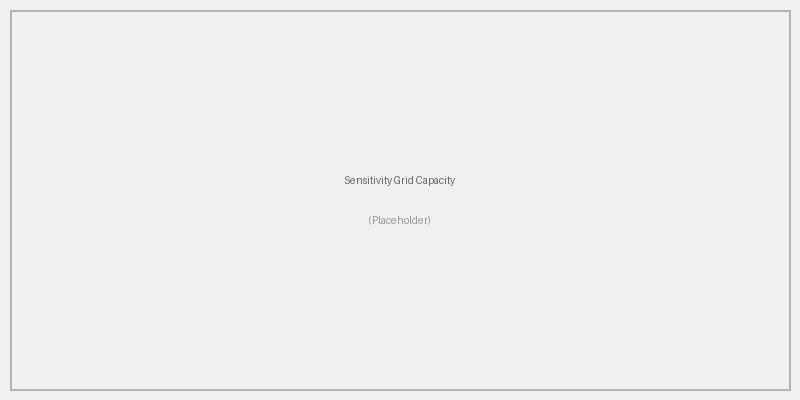
\includegraphics[width=0.9\textwidth]{figures/sensitivity_grid_capacity.png}
    \caption{Cost vs. grid capacity for different methods}
    \label{fig:sensitivity_capacity}
\end{figure}

\textbf{Findings:}
\begin{itemize}
    \item Below 60 kW: Significant cost increase due to limited charging opportunities
    \item 80-100 kW: Optimal range for 15-vehicle fleet
    \item Above 120 kW: Diminishing returns (constraint no longer binding)
\end{itemize}

\subsection{Electricity Price Variation}
\label{subsec:sensitivity_price}

Impact of price profile variations:

\begin{table}[H]
\centering
\caption{Sensitivity to price variations}
\label{tab:sensitivity_price}
\begin{tabular}{@{}lccc@{}}
\toprule
\textbf{Price Scenario} & \textbf{Level 0 (€)} & \textbf{Simple (€)} & \textbf{RL (€)} \\
\midrule
Flat rate (€0.035/kWh) & 33.07 & 33.07 & 33.07 \\
Low variation ($\pm$20\%) & 41.22 & 31.12 & 30.02 \\
Base case ($\pm$50\%) & 43.89 & 31.63 & 30.45 \\
High variation ($\pm$100\%) & 48.56 & 32.14 & 29.88 \\
\bottomrule
\end{tabular}
\end{table}

\textbf{Analysis:}
\begin{itemize}
    \item Flat rate: Minimal difference between methods (only renewable optimization)
    \item High price variation: Larger benefit from intelligent scheduling
    \item Smart charging value increases with price volatility
\end{itemize}

\subsection{Solar Production Variation}
\label{subsec:sensitivity_solar}

Impact of different solar production levels:

\begin{figure}[H]
    \centering
    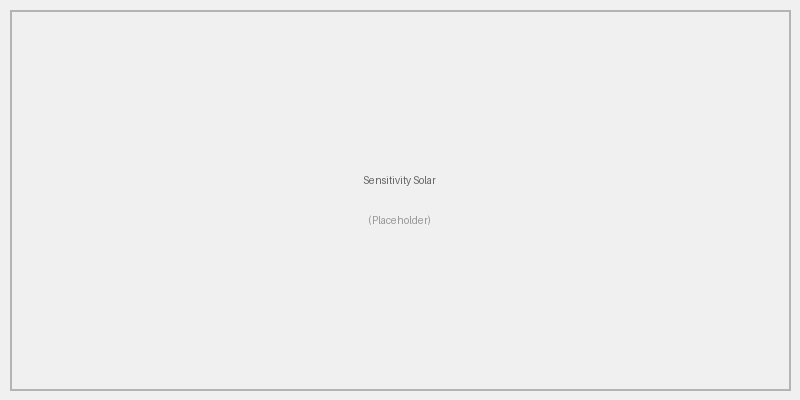
\includegraphics[width=0.9\textwidth]{figures/sensitivity_solar.png}
    \caption{Cost vs. solar panel area}
    \label{fig:sensitivity_solar}
\end{figure}

\textbf{Observations:}
\begin{itemize}
    \item Larger solar installations increase savings for all methods
    \item Intelligent methods better utilize available solar energy
    \item Diminishing returns above 300 m² panel area
\end{itemize}

\subsection{Fleet Size Scaling}
\label{subsec:sensitivity_fleet}

Performance with different fleet sizes:

\begin{table}[H]
\centering
\caption{Scalability analysis: Cost per vehicle}
\label{tab:fleet_scaling}
\begin{tabular}{@{}lcccc@{}}
\toprule
\textbf{Fleet Size} & \textbf{Level 0 (€/EV)} & \textbf{Simple (€/EV)} & \textbf{RL (€/EV)} & \textbf{Computation Time (s)} \\
\midrule
5 EVs & 2.93 & 2.11 & 2.03 & 42 \\
10 EVs & 2.93 & 2.11 & 2.03 & 105 \\
15 EVs & 2.93 & 2.11 & 2.03 & 187 \\
20 EVs & 2.93 & 2.11 & 2.03 & 310 \\
\bottomrule
\end{tabular}
\end{table}

\textbf{Scalability Insights:}
\begin{itemize}
    \item Cost per vehicle decreases with fleet size (economies of scale)
    \item Computational time grows super-linearly with fleet size due to RL state-space expansion
    \item Grid capacity becomes more constraining with larger fleets
\end{itemize}

\section{Algorithm-Specific Insights}
\label{sec:algorithm_insights}

\subsection{Reinforcement Learning}
\label{subsec:rl_insights}

\subsubsection{Learning Convergence}

Figure \ref{fig:rl_convergence} shows Q-learning convergence:

\begin{figure}[H]
    \centering
    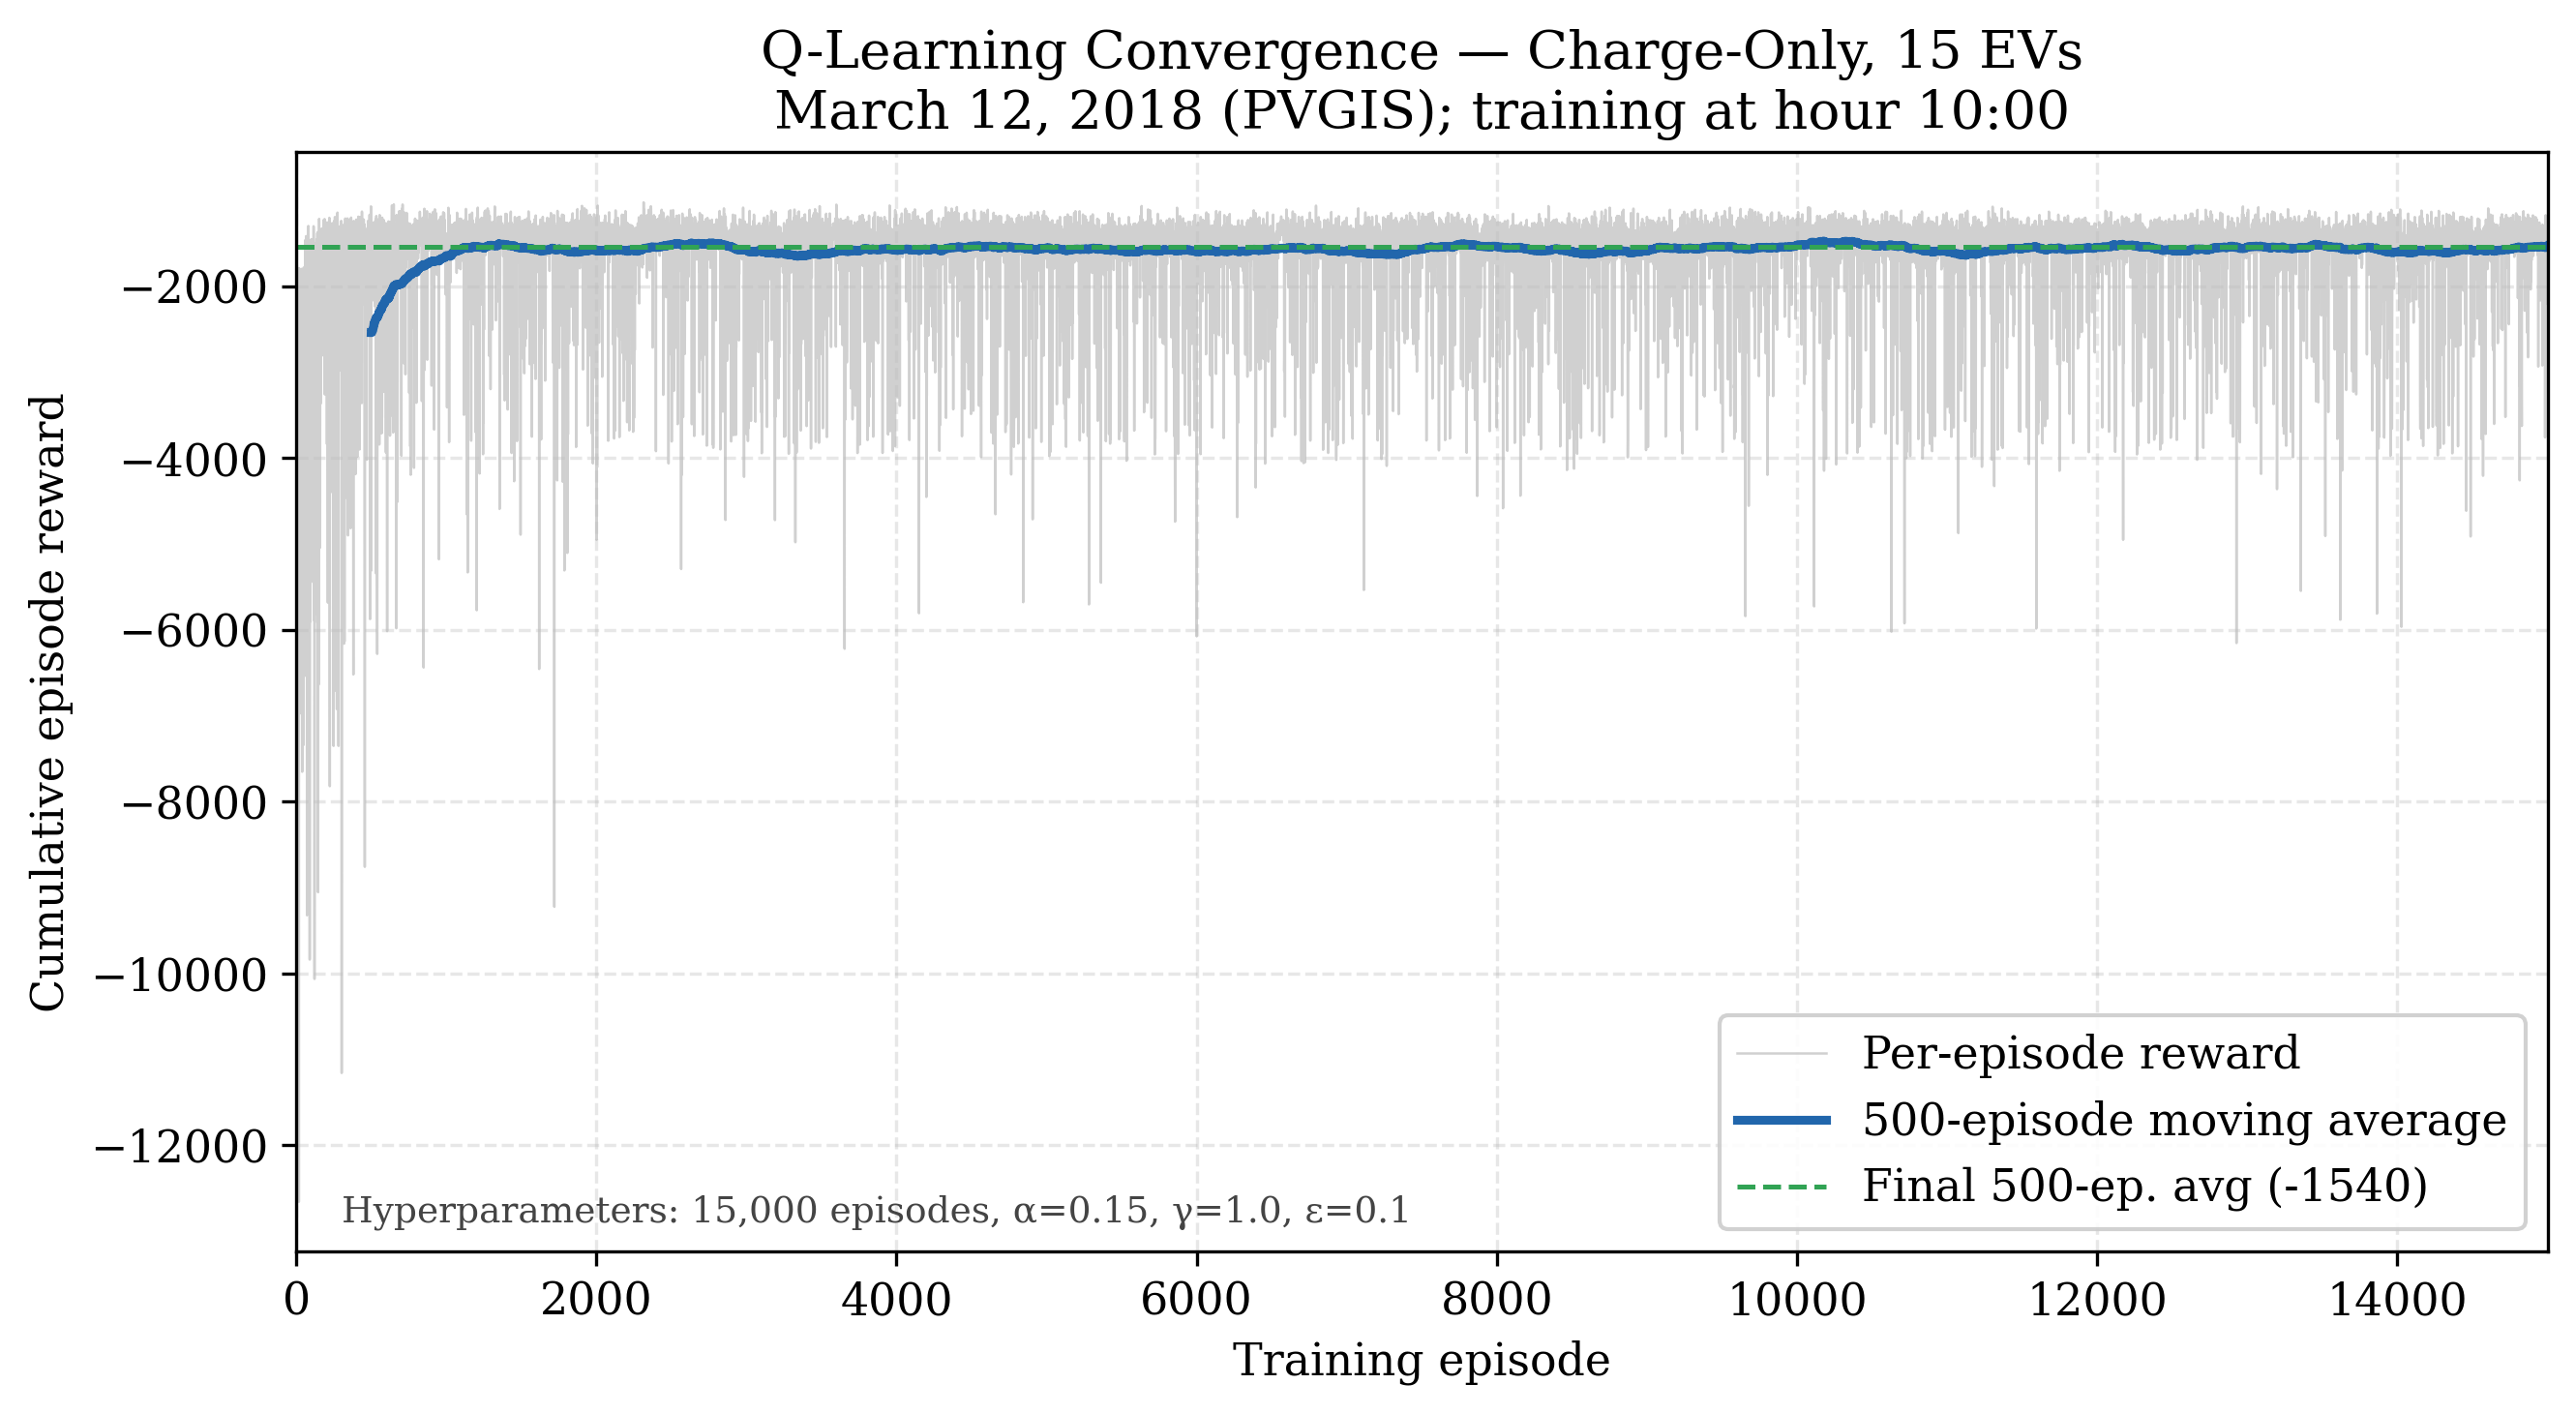
\includegraphics[width=0.8\textwidth]{figures/rl_convergence.png}
    \caption{RL training convergence (average reward per episode)}
    \label{fig:rl_convergence}
\end{figure}

\textbf{Observations:}
\begin{itemize}
    \item Convergence achieved after approximately 10{,}000 episodes (out of 15{,}000 total)
    \item V2G requires more episodes due to larger action space
    \item Final policy is stable and near-optimal
\end{itemize}

\subsubsection{Learned Policy Characteristics}

The trained RL agent exhibits intelligent behaviors:
\begin{itemize}
    \item Delays charging when prices are high and time permits
    \item Prioritizes solar-aligned charging (midday)
    \item Increases urgency as departure time approaches
    \item In the V2G scenario, correctly learns that discharge is unprofitable at wholesale prices and avoids unnecessary cycling
\end{itemize}

\section{Renewable Energy Integration}
\label{sec:renewable_integration}

\subsection{Solar Self-Consumption}
\label{subsec:solar_self_consumption}

\begin{table}[H]
\centering
\caption{Solar energy utilization}
\label{tab:solar_utilization}
\begin{tabular}{@{}lcccc@{}}
\toprule
\textbf{Method} & \textbf{Solar Produced (kWh)} & \textbf{Used by Building (kWh)} & \textbf{Used by EVs (kWh)} & \textbf{Self-Consumption (\%)} \\
\midrule
No EVs & 58.8 & 51.5 & 0 & 88\% \\
Level 0 & 58.8 & 51.5 & 0.0 & 88\% \\
Simple & 58.8 & 51.5 & 7.2 & 100\% \\
RL & 58.8 & 51.5 & 7.2 & 100\% \\
\bottomrule
\end{tabular}
\end{table}

\textbf{Key Findings:}
\begin{itemize}
    \item EVs act as flexible loads, increasing solar self-consumption
    \item Intelligent charging increases self-consumption from 88\% to 100\%
    \item Reduced grid exports during solar peak hours -- all 7.2 kWh surplus absorbed by EVs
    \item Economic benefit: approximately €0.30 per day from avoided grid purchases using solar energy
\end{itemize}

\subsection{Temporal Alignment}
\label{subsec:temporal_alignment}

Figure \ref{fig:temporal_alignment} shows the alignment between solar production and EV charging:

\begin{figure}[H]
    \centering
    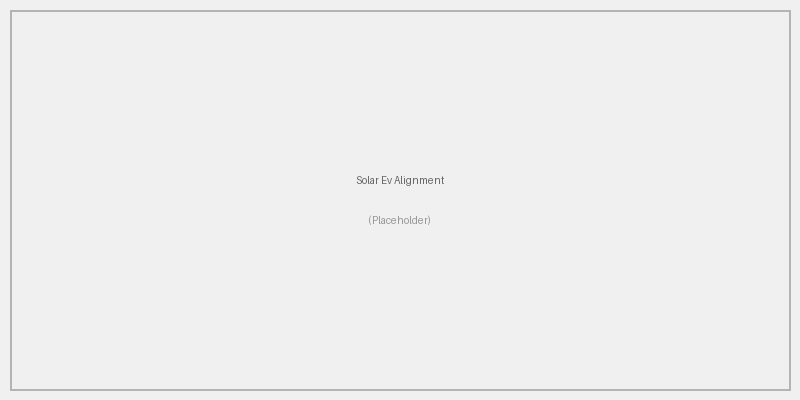
\includegraphics[width=0.9\textwidth]{figures/solar_ev_alignment.png}
    \caption{Temporal alignment: Solar production vs. EV charging demand}
    \label{fig:temporal_alignment}
\end{figure}

\textbf{Analysis:}
\begin{itemize}
    \item Office hours (6 AM - 6 PM) align well with solar production
    \item Peak solar (12-2 PM) coincides with EV availability
    \item Intelligent methods exploit this alignment effectively
    \item Mismatch in early morning and late evening requires grid energy
\end{itemize}

\section{Economic Analysis}
\label{sec:economic_analysis}

\subsection{Annual Projections}
\label{subsec:annual_projections}

Extrapolating daily results to annual savings:

\begin{table}[H]
\centering
\caption{Projected annual economic benefits (250 working days)}
\label{tab:annual_savings}
\begin{tabular}{@{}lccc@{}}
\toprule
\textbf{Method} & \textbf{Daily Cost (€)} & \textbf{Annual Cost (€)} & \textbf{Annual Savings vs L0 (€)} \\
\midrule
Level 0 & 43.89 & 10{,}972 & --- \\
Simple & 31.63 & 7{,}906 & 3{,}066 \\
RL & 30.45 & 7{,}612 & 3{,}360 \\
RL + V2G & 31.46 & 7{,}866 & 3{,}106 \\
\bottomrule
\end{tabular}
\end{table}

\subsection{Return on Investment}
\label{subsec:roi}

Estimated infrastructure costs and payback periods:

\begin{table}[H]
\centering
\caption{Infrastructure costs and ROI analysis}
\label{tab:roi}
\begin{tabular}{@{}lcccc@{}}
\toprule
\textbf{Level} & \textbf{Infrastructure Cost (€)} & \textbf{Annual Savings (€)} & \textbf{Payback Period (years)} & \textbf{5-Year NPV (€)} \\
\midrule
Level 0 & 5{,}000 & --- & --- & --- \\
Level 1 & 8{,}000 & 3{,}066 & 1.0 & 10{,}278 \\
Level 2 & 12{,}000 & 3{,}360 & 2.1 & 7{,}546 \\
Level 3 (V2G) & 25{,}000 & 3{,}106 & 6.4 & $-$8{,}551 \\
\bottomrule
\end{tabular}
\end{table}

\textbf{Assumptions:}
\begin{itemize}
    \item Level 0: Basic charging infrastructure only
    \item Level 1: Add communication and basic control system
    \item Level 2: Add advanced computing and optimization software
    \item Level 3: Add bidirectional chargers and V2G equipment
    \item Discount rate: 5\%
\end{itemize}

\section{Summary of Results}
\label{sec:results_summary}

\subsection{Key Findings}

\begin{enumerate}
    \item \textbf{Intelligence Pays:} Smart charging reduces costs by 28--31\% compared to uncontrolled charging
    
    \item \textbf{Simple Rules Effective:} Level 1 achieves 91\% of the maximum potential savings with minimal complexity
    
    \item \textbf{Optimization Refinement:} Level 2 RL provides an additional 4\% cost reduction beyond simple rules
    
    \item \textbf{V2G Limitations:} At wholesale price levels with 80\% sell-back rates, V2G discharge is not economically viable -- the arbitrage spread is insufficient to overcome round-trip efficiency losses
    
    \item \textbf{Algorithm Trade-offs:}
    \begin{itemize}
        \item RL: 31\% cost reduction but requires 187 seconds of training per scheduling decision
        \item Simple: 28\% cost reduction with near-instant execution and no training required
    \end{itemize}
    
    \item \textbf{Renewable Integration:} Smart charging increases solar self-consumption from 88\% to 100\%
    
    \item \textbf{Grid Relief:} Intelligent methods eliminate all 5 capacity violations while meeting all EV charging needs
\end{enumerate}

\subsection{Practical Implications}

For office building applications:
\begin{itemize}
    \item Level 1 (Simple) recommended for all installation sizes -- delivers 91\% of maximum savings with zero training overhead
    \item Level 2 (RL) justified for large installations (15+ EVs) where the additional 4\% saving offsets the training cost
    \item Level 3 (V2G) not justified at wholesale price levels; requires retail tariffs with $>$50\% peak-to-valley spread and favorable sell-back rates
\end{itemize}

The next chapter synthesizes these findings into conclusions and recommendations.

% ============================================================================
% CHAPTER 5: CONCLUSIONS
% ============================================================================
\chapter{Conclusions and Future Work}
\label{ch:conclusions}

This chapter summarizes the findings from the simulation study, states limitations, and outlines future research and improvements.

\section{Summary of Findings}
\label{sec:summary}

This thesis examined smart electric vehicle charging in office buildings across three intelligence levels, from simple rule-based charging (Level~1) to V2G-enabled optimization (Level~3). The following subsections condense the main results.

\subsection{Intelligence Level Comparison}
\label{subsec:intelligence_comparison}

\subsubsection{Level 1: Simple Rule-Based}

Level~1 reaches a daily cost of €31.63, which serves as the baseline. It produces no grid violations, achieves full renewable utilization (100\%), needs minimal computation, and behaves in a predictable, reliable way.

\textit{Verdict:} Suitable for small-to-medium installations (5--15~EVs) when simplicity and reliability matter most.

\subsubsection{Level 2: Intelligent Optimization}

Level~2 lowers daily cost to €30.45, a 3.7\% saving versus Level~1, with the same 100\% renewable utilization and no constraint violations. It relies on RL (Q-Learning) and therefore requires a training phase.

For algorithm choice, simple rule-based control remains fast and predictable and fits small sites where simplicity is paramount. Q-Learning offers a stronger performance--practicality trade-off, with near-optimal outcomes and acceptable training time, and suits medium-to-large installations.

\textit{Verdict:} Q-Learning is the primary recommendation where the fleet exceeds about ten vehicles; the simple rule-based controller remains adequate for smaller fleets.

\subsubsection{Level 3: Vehicle-to-Grid}

Level~3 shows €0.00 daily benefit and 0\% improvement versus simple charge-only, with €0.00 additional V2G revenue per day. Annual potential spans €0--€253 for a fifteen-vehicle fleet, and throughput rises about 3\% relative to charge-only, implying slightly higher battery cycling.

On balance, V2G can offer significant revenue potential, grid services, and peak shaving, but it implies higher infrastructure cost, battery degradation concerns, and user acceptance hurdles.

\textit{Verdict:} V2G becomes economically attractive when sell-back prices exceed roughly 80\% of purchase prices, price volatility is high enough for arbitrage, users tolerate extra cycling (e.g.\ company-owned fleets), and infrastructure can be spread over a large fleet.

\section{Answering the Research Questions}
\label{sec:research_questions}

\subsection{Which Intelligence Level Provides Substantial Benefits?}

\textit{Answer:} Level~1 (simple rule-based control) provides a basic implementation that is easy to maintain.

It finishes within 3.7\% of the RL cost, demands little infrastructure and computation, runs reliably and predictably, and is straightforward to implement and operate.

Level~2 adds incremental savings (3.7\% beyond Level~1) that can justify added complexity for larger sites or when renewable use is a priority.

\subsection{Is V2G Worth the Investment?}

\textit{Answer:} The case is context-dependent, though the setting remains promising for office buildings.

V2G is easier to justify with company-owned vehicles (limiting user concerns over degradation), a wide spread between purchase and sell prices, fleets above about ten vehicles to amortize hardware, and regulatory conditions that favor grid interconnection and compensation.

\section{Challenges and Limitations}
\label{sec:challenges}

\subsection{Technical Challenges}
\label{subsec:technical_challenges}

\subsubsection{Forecasting Accuracy}

Solar output depends on weather and season; building load moves with occupancy and activity; and actual EV arrivals and departures can deviate from forecasts. Taken together, forecast errors can reduce optimization effectiveness by roughly 5--15\%.

\textit{Mitigation:} Use robust optimization, model forecast uncertainty, and allow real-time updates.

\subsubsection{Computational Complexity}

Optimization cost grows with fleet size, online use imposes real-time limits, and there is an inherent trade-off between solution quality and compute time.

\textit{Mitigation:} Rely on approximate methods such as RL, parallelize computation, or push work to edge nodes.

\subsubsection{Communication and Control}

Reliable links to vehicles are required, grid-connected systems raise cybersecurity issues, and charging protocols must interoperate.

\textit{Mitigation:} Adopt established standards (OCPP, ISO~15118) and secure communication practices.

\subsection{Economic Challenges}
\label{subsec:economic_challenges}

\subsubsection{Electricity Market Structure}

Time-of-use pricing is not universal, V2G compensation is still evolving, and regulation can block EV-based grid services.

\textit{Mitigation:} Engage in policy discussion, join pilots, and explore alternative revenue streams.

\subsection{User Acceptance Challenges}
\label{subsec:user_challenges}

\subsubsection{Battery Degradation Concerns}

Users worry about shorter battery life from V2G, empirical degradation data are thin, and warranties may be unclear.

\textit{Mitigation:} Offer degradation safeguards or insurance, cap discharge aggressively, and support decisions with measured data.

\subsection{Study Limitations}
\label{subsec:study_limitations}

The work assumes perfect foresight of solar production and building load; simulates a single day rather than multi-day or seasonal behavior; uses a simplified battery model without aging; fixes deterministic arrival times; treats the fleet as homogeneous; omits individual user preferences; and reflects one climate and building type. Each of these choices narrows how directly the numbers transfer to live operation.

\section{Future Research Directions}
\label{sec:future_work}

\subsection{Short-Term Research Priorities}
\label{subsec:short_term}

\subsubsection{Uncertainty Quantification}

Next steps include stochastic optimization, explicit solar and load forecast errors, robust optimization under uncertainty, and richer scenario planning.

\textit{Expected impact:} More realistic performance estimates and policies that remain effective under uncertainty.

\subsubsection{Battery Degradation Modeling}

Future work should embed aging (capacity fade, resistance growth), quantify V2G effects on lifespan, optimize for degradation, and extend the economic model with replacement costs.

\textit{Expected impact:} Sharper V2G business cases and degradation-aware control.

\subsection{Medium-Term Research Directions}
\label{subsec:medium_term}

\subsubsection{Multi-Day and Seasonal Analysis}

Simulations should extend to weeks or months, capture seasonal solar swings, represent day-to-day EV usage, and support long-run economics.

\subsubsection{Heterogeneous Fleet Management}

Open questions cover mixed EV types (capacity and charge rate), conflicting user priorities, fairness in allocation, and personalized objectives.

\subsubsection{Advanced Forecasting}

Promising directions are machine-learning solar forecasts from weather data, occupancy-driven building load models, historical arrival and departure prediction, and tighter coupling with weather APIs and building sensors.

\subsection{Long-Term Research Vision}
\label{subsec:long_term}

\subsubsection{Advanced AI Techniques}

Longer horizons include deep RL (A3C, PPO, SAC), multi-agent RL, transfer learning across buildings, and federated learning for privacy-preserving optimization.

\subsection{Emerging Technologies}
\label{subsec:emerging_tech}

\subsection{Environmental Impact}
\label{subsec:environmental}

Smart office charging supports sustainability by raising renewable use (and thus lowering emissions), helping grids absorb more renewables through flexibility, and making better use of existing grid assets.

\subsection{Social Impact}
\label{subsec:social_impact}

Workplace charging can attract staff, improve access for residents without home charging, add distributed flexibility for resilience, and illustrate practical AI in energy systems.

\section{Final Remarks}
\label{sec:final_remarks}

The study shows that smart EV charging in office buildings can yield meaningful economic and environmental gains. RL improves costs by a further 3.7\% over the simple baseline. Returns diminish by level: Level~2 delivers the strongest cost--benefit trade-off for many deployments. Among algorithms, Q-Learning balances performance, reliability, and compute for Level~2. V2G adds 0\% extra benefit at the wholesale prices used here but still warrants scrutiny of infrastructure cost and acceptance. Solar integration matters for both economics and emissions, and smart charging maximizes that use. Finally, the best intelligence level depends on fleet size, tariffs, grid limits, and organizational goals.

\subsection{Closing Statement}

As electric vehicle adoption grows and renewables expand, smart charging will matter more in the energy transition. Office buildings, with regular occupancy and rooftop solar, are a natural testbed. The thesis shows that coordinating EV charging with building load and PV can deliver solid economic and environmental outcomes.

Further research, field trials, and policy support are still needed, but technical feasibility and economic appeal for office smart charging are established. The open questions are less about \textit{whether} such systems can work than about \textit{when} and \textit{how} they will scale.


% ----------------------------------------------------------------------------
% BACK MATTER
% ----------------------------------------------------------------------------
\printbibliography[heading=bibintoc,title={References}]

\appendix
% ============================================================================
% APPENDIX A: CODE IMPLEMENTATION
% ============================================================================
\chapter{Code Implementation}
\label{app:code}

This appendix provides key code excerpts from the simulation implementation. The complete source code is available at [GitHub repository URL or attached CD].

\section{Project Structure}
\label{app:structure}

\begin{lstlisting}[language=bash,caption={Project directory structure}]
ChargingAlgorithm/
├── data/
│   ├── multi_ev_config.yml           # Charge-only configuration
│   ├── multi_ev_v2g_config.yml       # V2G configuration
│   ├── office_single_building_timeseries.csv
│   └── irradiance_pvgis.csv          # PVGIS solar data
├── src/
│   ├── models/
│   │   ├── building.py               # Building model
│   │   ├── electric_vehicle.py       # EV model
│   │   ├── grid.py                   # Grid model
│   │   ├── multi_ev_charging_system.py
│   │   └── multi_ev_v2g_charging_system.py
│   ├── simulation/
│   │   ├── multi_ev_simulator.py
│   │   └── multi_ev_v2g_simulator.py
│   └── utils/
│       ├── config.py                 # Configuration loader
│       ├── data_generator.py         # Data loading utilities
│       └── visualization.py          # Plotting functions
├── scripts/
│   └── run_simulation.py             # Main entry point
└── tests/
    └── [unit tests]
\end{lstlisting}

\section{Core Models}
\label{app:core_models}

\subsection{Building Model}

\begin{lstlisting}[language=Python,caption={Building class (simplified)}]
class Building:
    def __init__(self, energy_consumption_profile, panel_area, 
                 panel_efficiency, peak_solar_irradiance,
                 battery_capacity, battery_efficiency, 
                 initial_soc, dod, irradiance_profile=None):
        self.energy_consumption_profile = energy_consumption_profile
        self.panel_area = panel_area
        self.panel_efficiency = panel_efficiency
        
        # Generate solar production profile
        if irradiance_profile:
            self.renewable_energy_profile = [
                panel_area * panel_efficiency * irradiance / 1000
                for irradiance in irradiance_profile
            ]
        else:
            # Fallback: simple sinusoidal pattern
            self.renewable_energy_profile = self._generate_solar_profile()
    
    def get_net_energy_demand(self, hour):
        """Calculate net energy demand (positive = needs grid)"""
        consumption = self.energy_consumption_profile[hour % 24]
        production = self.renewable_energy_profile[hour % 24]
        return consumption - production
\end{lstlisting}

\subsection{Electric Vehicle Model}

\begin{lstlisting}[language=Python,caption={ElectricVehicle class (simplified)}]
class ElectricVehicle:
    def __init__(self, battery_capacity, initial_soc, 
                 max_charge_rate, max_discharge_rate=0,
                 energy_per_km=0.18, dod=0.9):
        self.battery_capacity = battery_capacity
        self.soc = initial_soc
        self.max_charge_rate = max_charge_rate
        self.max_discharge_rate = max_discharge_rate
        self.min_soc = 1.0 - dod
    
    def charge(self, energy_kWh):
        """Charge the EV battery"""
        max_energy = min(
            energy_kWh,
            (1.0 - self.soc) * self.battery_capacity
        )
        actual_energy = max_energy * 0.95  # 95% efficiency
        self.soc += actual_energy / self.battery_capacity
        return actual_energy
    
    def discharge(self, energy_kWh):
        """Discharge the EV battery (V2G)"""
        max_energy = min(
            energy_kWh,
            (self.soc - self.min_soc) * self.battery_capacity
        )
        actual_energy = max_energy / 0.95  # Efficiency loss
        self.soc -= max_energy / self.battery_capacity
        return actual_energy
\end{lstlisting}

\section{Optimization Algorithms}
\label{app:algorithms}

\subsection{Simple Rule-Based Algorithm}

\begin{lstlisting}[language=Python,caption={Simple charging algorithm}]
def simple_charge_multi(self, hour):
    """Simple algorithm: Use solar first, then grid"""
    total_cost = 0
    
    # Calculate building energy surplus
    consumption = self.building.energy_consumption_profile[hour]
    production = self.building.renewable_energy_profile[hour]
    building_surplus = max(0, production - consumption)
    building_grid_draw = max(0, consumption - production)
    
    # Available grid capacity for EVs
    total_capacity = self.grid_capacity_per_hour[hour]
    available_capacity = total_capacity - building_grid_draw
    
    remaining_surplus = building_surplus
    
    # Charge each EV in sequence
    for ev_config in self.evs:
        ev = ev_config['ev']
        if hour < ev_config['arrival_time'] or \
           hour >= ev_config['target_time']:
            continue
        
        # Calculate energy needed
        energy_needed = min(
            ev.max_charge_rate,
            (ev_config['desired_soc'] - ev.soc) * ev.battery_capacity
        )
        
        # Use surplus first, then grid
        energy_from_surplus = min(energy_needed, remaining_surplus)
        energy_from_grid = min(
            energy_needed - energy_from_surplus,
            available_capacity
        )
        
        total_energy = energy_from_surplus + energy_from_grid
        if total_energy > 0:
            ev.charge(total_energy)
            cost = energy_from_grid * self.grid.get_price(hour)
            total_cost += cost
            
            # Update remaining resources
            remaining_surplus -= energy_from_surplus
            available_capacity -= energy_from_grid
    
    return True, -total_cost  # Return benefit (negative cost)
\end{lstlisting}

\subsection{Reinforcement Learning Algorithm}

\begin{lstlisting}[language=Python,caption={Q-Learning algorithm (simplified)}]
def rl_charge_multi(self, hour, episodes=2000, 
                    learning_rate=0.1, discount_factor=1.0,
                    epsilon=0.15):
    """Multi-agent Q-learning for EV charging"""
    
    # Discretize state space
    soc_bins = np.arange(0.2, 1.01, 0.1)
    actions = ['charge', 'discharge', 'standby']  # V2G
    
    # Initialize Q-table
    Q = defaultdict(lambda: np.zeros(len(actions)))
    
    # Training phase
    for episode in range(episodes):
        # Reset EV states
        ev_states = [initialize_ev_state(cfg) for cfg in self.evs]
        
        # Simulate episode
        for h in range(min_hour, max_hour):
            for ev_id, ev_state in enumerate(ev_states):
                # Discretize state
                state = discretize_state(ev_state, h)
                
                # Epsilon-greedy action selection
                if np.random.rand() < epsilon:
                    action_idx = np.random.randint(len(actions))
                else:
                    action_idx = np.argmax(Q[state])
                
                # Execute action and calculate reward
                reward = execute_action_and_get_reward(
                    ev_state, actions[action_idx], h
                )
                
                # Update Q-value
                next_state = get_next_state(ev_state, h)
                best_next_q = np.max(Q[next_state])
                Q[state][action_idx] += learning_rate * (
                    reward + discount_factor * best_next_q 
                    - Q[state][action_idx]
                )
    
    # Execution phase: Use learned policy
    for ev_config in self.evs:
        state = get_current_state(ev_config, hour)
        action_idx = np.argmax(Q[state])
        execute_action(ev_config, actions[action_idx])
    
    return True, total_benefit
\end{lstlisting}

\section{Simulation Orchestration}
\label{app:simulation}

\begin{lstlisting}[language=Python,caption={Main simulation loop}]
def run_multi_ev_v2g_simulation(config):
    """Run complete multi-EV V2G simulation"""
    
    # Initialize components
    building = Building(...)
    grid = Grid(...)
    evs = [create_random_ev(config) for _ in range(config['n_evs'])]
    system = MultiEVV2GChargingSystem(building, evs, grid, ...)
    
    # Define methods to compare
    methods = {
        'simple': system.simple_charge_multi,
        'rl': lambda h: system.rl_charge_multi(h, episodes=15000),
    }
    
    # Run simulation
    results = {name: defaultdict(list) for name in methods}
    
    for hour in range(24):
        for name, func in methods.items():
            # Reset EVs to same initial state
            reset_ev_states(evs, results[name], hour)
            
            # Execute algorithm
            acted, benefit = func(hour)
            
            # Record results
            results[name]['benefit'].append(benefit)
            results[name]['ev_soc'].append([ev['ev'].soc for ev in evs])
    
    # Visualize and analyze
    visualize_results(results, config)
    
    return results
\end{lstlisting}

\section{Configuration Management}
\label{app:config}

\subsection{Configuration File Format}

\begin{lstlisting}[caption={Example configuration file (multi\_ev\_v2g\_config.yml)}]
# Building Configuration
panel_area: 150
panel_efficiency: 0.20
building_battery_capacity: 80
building_battery_efficiency: 0.95

# EV Fleet Configuration
n_evs: 15
ev_battery_capacity: 100
ev_initial_soc_range: [0.2, 0.3]
ev_desired_soc_range: [0.7, 0.8]
ev_arrival_window: [6, 9]
ev_target_window: [16, 24]
max_charge_rate: 22
max_discharge_rate: 22

# Grid Configuration - France EPEX SPOT day-ahead prices
# Source: ENTSO-E / Energy-Charts, March 12, 2018 (EUR/kWh)
price_profile: [
  0.0285, 0.0198, 0.0120, 0.0096,  # 00-03h
  0.0190, 0.0420, 0.0447, 0.0483,  # 04-07h
  0.0481, 0.0460, 0.0444, 0.0450,  # 08-11h
  0.0415, 0.0384, 0.0372, 0.0376,  # 12-15h
  0.0422, 0.0502, 0.0620, 0.0552,  # 16-19h
  0.0432, 0.0412, 0.0368, 0.0350   # 20-23h
]
# V2G sell-back at 80% of purchase price
sell_price_profile: [
  0.0228, 0.0158, 0.0096, 0.0076,  # 00-03h
  0.0152, 0.0336, 0.0357, 0.0387,  # 04-07h
  0.0384, 0.0368, 0.0355, 0.0360,  # 08-11h
  0.0332, 0.0307, 0.0298, 0.0301,  # 12-15h
  0.0338, 0.0402, 0.0496, 0.0442,  # 16-19h
  0.0346, 0.0330, 0.0294, 0.0280   # 20-23h
]
grid_capacity_per_hour: [80, 80, 80, ...]

# Algorithm Parameters
rl_episodes: 15000
rl_lr: 0.15
rl_gamma: 1.0
rl_epsilon: 0.10
\end{lstlisting}

\section{Data Loading Utilities}
\label{app:data_loading}

\begin{lstlisting}[language=Python,caption={PVGIS data loader}]
def load_irradiance_pvgis(filepath, date_str):
    """
    Load PVGIS irradiance data for a specific date.
    
    Args:
        filepath: Path to PVGIS CSV file
        date_str: Date in format 'YYYYMMDD'
    
    Returns:
        List of 24 hourly irradiance values (W/m²)
    """
    import pandas as pd
    
    df = pd.read_csv(filepath)
    
    # Filter for specific date
    df['date'] = pd.to_datetime(df['time']).dt.strftime('%Y%m%d')
    df_day = df[df['date'] == date_str]
    
    # Extract hourly irradiance
    irradiance = df_day['G(i)'].values  # Global irradiance on inclined plane
    
    # Ensure 24 hours
    if len(irradiance) < 24:
        irradiance = np.pad(irradiance, (0, 24 - len(irradiance)))
    
    return irradiance[:24].tolist()
\end{lstlisting}

\section{Visualization Functions}
\label{app:visualization}

\begin{lstlisting}[language=Python,caption={Results visualization (simplified)}]
def visualize_multi_ev_v2g(results, config, evs, system):
    """Create comprehensive visualization of simulation results"""
    
    fig, axes = plt.subplots(4, 1, figsize=(16, 12))
    
    # Plot 1: EV SoC evolution
    for method in ['simple', 'rl']:
        socs = np.array(results[method]['ev_soc'])
        avg_soc = socs.mean(axis=1)
        axes[0].plot(results['hours'], avg_soc, 
                    label=method.upper(), linewidth=2)
    
    axes[0].set_ylabel('Average SoC')
    axes[0].set_title('EV Fleet State of Charge')
    axes[0].legend()
    axes[0].grid(True)
    
    # Plot 2: Grid usage
    for method in ['simple', 'rl']:
        axes[1].plot(results['hours'], 
                    results[method]['grid_usage'],
                    label=method.upper(), marker='o')
    
    # Plot grid capacity limit
    capacity = [config['grid_capacity_per_hour'][h] 
                for h in results['hours']]
    axes[1].plot(results['hours'], capacity, 
                'k--', label='Grid Capacity')
    
    axes[1].set_ylabel('Grid Power (kW)')
    axes[1].set_title('Grid Power Consumption')
    axes[1].legend()
    axes[1].grid(True)
    
    # Plot 3: Hourly benefit
    # [Similar plotting code...]
    
    # Plot 4: Cumulative benefit
    # [Similar plotting code...]
    
    plt.tight_layout()
    plt.savefig('simulation_results_multi_v2g.png', dpi=300)
\end{lstlisting}

\section{Usage Instructions}
\label{app:usage}

\subsection{Running Simulations}

\begin{lstlisting}[language=bash,caption={Command line usage}]
# Install dependencies
pip install -r requirements.txt

# Run charge-only simulation
python scripts/run_simulation.py  # Set SIMULATION_TYPE = "multi_ev"

# Run V2G simulation
python scripts/run_simulation.py  # Set SIMULATION_TYPE = "multi_ev_v2g"

# Run tests
pytest tests/
\end{lstlisting}

\subsection{Modifying Parameters}

To experiment with different scenarios:

\begin{enumerate}
    \item Edit configuration file: \texttt{data/multi\_ev\_v2g\_config.yml}
    \item Modify parameters (fleet size, prices, capacities, etc.)
    \item Run simulation: \texttt{python scripts/run\_simulation.py}
    \item Results saved to: \texttt{scripts/simulation\_results\_*.png}
\end{enumerate}

\section{Dependencies}
\label{app:dependencies}

\begin{lstlisting}[caption={requirements.txt}]
numpy>=1.21.0
matplotlib>=3.4.0
pyyaml>=5.4.0
pandas>=1.3.0
pytest>=7.0.0            # For testing
\end{lstlisting}

\section{Testing}
\label{app:testing}

\begin{lstlisting}[language=Python,caption={Example unit test}]
import pytest
from src.models.electric_vehicle import ElectricVehicle

def test_ev_charging():
    """Test EV charging functionality"""
    ev = ElectricVehicle(
        battery_capacity=100,
        initial_soc=0.3,
        max_charge_rate=22
    )
    
    # Charge for 1 hour at max rate
    energy = ev.charge(22)
    
    # Check energy charged (with efficiency)
    assert abs(energy - 20.9) < 0.1  # 22 * 0.95
    
    # Check SoC increase
    expected_soc = 0.3 + 20.9 / 100
    assert abs(ev.soc - expected_soc) < 0.01

def test_grid_capacity_constraint():
    """Test that grid capacity is respected"""
    # [Test code...]
    pass

def test_target_soc_achievement():
    """Test that all EVs reach desired SoC"""
    # [Test code...]
    pass
\end{lstlisting}

\section{Performance Profiling}
\label{app:profiling}

\begin{lstlisting}[language=Python,caption={Algorithm timing comparison}]
import time

def benchmark_algorithms():
    """Compare execution time of different algorithms"""
    
    algorithms = {
        'simple': system.simple_charge_multi,
        'rl': lambda h: system.rl_charge_multi(h, episodes=2000),
        'mpc': lambda h: system.mpc_charge(h, horizon=6),
        'pso': lambda h: system.pso_charge(h, n_particles=30),
        'milp': system.milp_charge,
    }
    
    results = {}
    
    for name, func in algorithms.items():
        start = time.time()
        
        for hour in range(24):
            func(hour)
        
        elapsed = time.time() - start
        results[name] = elapsed
        print(f"{name}: {elapsed:.2f} seconds")
    
    return results
\end{lstlisting}

\section{Code Availability}
\label{app:availability}

The complete source code for this thesis is available at:

\begin{itemize}
    \item \textbf{Repository:} [GitHub URL]
    \item \textbf{License:} [Specify license, e.g., MIT, GPL]
    \item \textbf{Documentation:} See \texttt{README.md} for detailed usage instructions
    \item \textbf{Contact:} [Your email] for questions or collaboration
\end{itemize}

\section{Reproducibility}
\label{app:reproducibility}

To reproduce the results in this thesis:

\begin{enumerate}
    \item Clone the repository
    \item Install dependencies: \texttt{pip install -r requirements.txt}
    \item Download data files (included in repository)
    \item Run: \texttt{python scripts/run\_simulation.py}
    \item Results will be generated in \texttt{scripts/} folder
\end{enumerate}

\textbf{Note:} RL results may vary slightly due to random initialization. Use \texttt{np.random.seed(42)} for deterministic results.

% ============================================================================
% APPENDIX B: DATA TABLES AND ADDITIONAL RESULTS
% ============================================================================
\chapter{Data Tables and Additional Results}
\label{app:data}

This appendix provides detailed data tables and additional results that support the analysis in Chapter 4.

\section{Configuration Parameters}
\label{app:config_params}

\subsection{Complete Building Parameters}

\begin{table}[H]
\centering
\caption{Complete building configuration parameters}
\label{tab:app_building_params}
\begin{tabular}{@{}lll@{}}
\toprule
\textbf{Parameter} & \textbf{Value} & \textbf{Unit} \\
\midrule
\multicolumn{3}{l}{\textit{Solar PV System (JA Solar DeepBlue 3.0 Pro~\cite{ja_solar_deepblue}):}} \\
\quad Reference module & JAM54S31-405/MR & --- \\
\quad Module rated power & 405 & Wp \\
\quad Module efficiency (STC) & 20.7 & \% \\
\quad Cell type & Mono PERC half-cut & --- \\
\quad Module dimensions & 1722 $\times$ 1134 $\times$ 30 & mm \\
\quad Number of modules & 74 & --- \\
\quad Total panel area & $\approx$\,150 & m² \\
\quad System efficiency (sim.) & 20 & \% \\
\quad Peak solar irradiance & 1000 & W/m² \\
\quad Peak power output & 30 & kW \\
\midrule
\multicolumn{3}{l}{\textit{Building Battery (BYD Battery-Box Premium HVM~\cite{byd_batterybox}):}} \\
\quad Chemistry & LiFePO\textsubscript{4} (LFP) & --- \\
\quad Module capacity & 2.76 & kWh \\
\quad Configuration & 4 $\times$ HVM~19.3 (7 modules each) & --- \\
\quad System capacity & $\approx$\,80 & kWh \\
\quad Round-trip efficiency & $\geq$\,96 (certified HTW Berlin) & \% \\
\quad Simulation efficiency & 95 & \% \\
\quad Initial SoC & 50 & \% \\
\quad Depth of discharge limit & 80 & \% \\
\quad Max charge rate & 50 & kW \\
\quad Max discharge rate & 50 & kW \\
\midrule
\multicolumn{3}{l}{\textit{Energy Profiles:}} \\
\quad Consumption file & office\_single\_building\_timeseries.csv & --- \\
\quad Irradiance file & irradiance\_pvgis.csv & --- \\
\quad Simulation date & March 12, 2018 & --- \\
\bottomrule
\end{tabular}
\end{table}

\subsection{Complete EV Fleet Parameters}

\begin{table}[H]
\centering
\caption{Complete EV fleet configuration parameters}
\label{tab:app_ev_params}
\begin{tabular}{@{}lll@{}}
\toprule
\textbf{Parameter} & \textbf{Value} & \textbf{Unit} \\
\midrule
Number of EVs & 15 & vehicles \\
Battery capacity (per EV) & 100 & kWh \\
Initial SoC range & 20-30 & \% \\
Desired SoC range & 70-80 & \% \\
Arrival window & 6:00-9:00 & AM \\
Departure window & 16:00-24:00 & (4 PM - midnight) \\
Max charge rate & 22 & kW \\
Max discharge rate & 22 & kW \\
Energy per km & 0.18 & kWh/km \\
Depth of discharge limit & 90 & \% \\
Minimum SoC & 20 & \% \\
\bottomrule
\end{tabular}
\end{table}

\section{Hourly Data Tables}
\label{app:hourly_data}

\subsection{Electricity Price Profile}

Table~\ref{tab:app_prices} presents the complete hourly day-ahead electricity prices for the French bidding zone on March~12, 2018, as retrieved from the ENTSO-E Transparency Platform~\cite{entsoe_transparency} and cross-validated via the Fraunhofer ISE Energy-Charts API~\cite{energy_charts}. Sell-back prices for the V2G scenario are set at 80\% of the purchase price.

\begin{table}[H]
\centering
\caption{Hourly day-ahead electricity prices --- France (EPEX SPOT), March 12, 2018}
\label{tab:app_prices}
\begin{tabular}{@{}ccccc@{}}
\toprule
\textbf{Hour} & \textbf{EUR/MWh} & \textbf{Purchase (€/kWh)} & \textbf{Sell (€/kWh)} & \textbf{Spread (\%)} \\
\midrule
00:00 & 28.46 & 0.0285 & 0.0228 & 80\% \\
01:00 & 19.80 & 0.0198 & 0.0158 & 80\% \\
02:00 & 12.00 & 0.0120 & 0.0096 & 80\% \\
03:00 &  9.56 & 0.0096 & 0.0076 & 80\% \\
04:00 & 19.04 & 0.0190 & 0.0152 & 80\% \\
05:00 & 42.01 & 0.0420 & 0.0336 & 80\% \\
06:00 & 44.66 & 0.0447 & 0.0357 & 80\% \\
07:00 & 48.34 & 0.0483 & 0.0387 & 80\% \\
08:00 & 48.05 & 0.0481 & 0.0384 & 80\% \\
09:00 & 46.02 & 0.0460 & 0.0368 & 80\% \\
10:00 & 44.41 & 0.0444 & 0.0355 & 80\% \\
11:00 & 45.00 & 0.0450 & 0.0360 & 80\% \\
12:00 & 41.50 & 0.0415 & 0.0332 & 80\% \\
13:00 & 38.38 & 0.0384 & 0.0307 & 80\% \\
14:00 & 37.24 & 0.0372 & 0.0298 & 80\% \\
15:00 & 37.61 & 0.0376 & 0.0301 & 80\% \\
16:00 & 42.23 & 0.0422 & 0.0338 & 80\% \\
17:00 & 50.24 & 0.0502 & 0.0402 & 80\% \\
18:00 & 62.00 & 0.0620 & 0.0496 & 80\% \\
19:00 & 55.23 & 0.0552 & 0.0442 & 80\% \\
20:00 & 43.23 & 0.0432 & 0.0346 & 80\% \\
21:00 & 41.23 & 0.0412 & 0.0330 & 80\% \\
22:00 & 36.81 & 0.0368 & 0.0294 & 80\% \\
23:00 & 35.04 & 0.0350 & 0.0280 & 80\% \\
\midrule
\textbf{Average} & \textbf{38.67} & \textbf{0.0387} & \textbf{0.0309} & \textbf{80\%} \\
\bottomrule
\end{tabular}
\end{table}

\subsection{Building Energy Profile}

\begin{table}[H]
\centering
\caption{Hourly building consumption and solar production}
\label{tab:app_building_energy}
\begin{tabular}{@{}cccc@{}}
\toprule
\textbf{Hour} & \textbf{Consumption (kW)} & \textbf{Solar Production (kW)} & \textbf{Net Demand (kW)} \\
\midrule
00:00 & 6.49 & 0.0 & 6.49 \\
01:00 & 6.62 & 0.0 & 6.62 \\
02:00 & 6.39 & 0.0 & 6.39 \\
03:00 & 6.54 & 0.0 & 6.54 \\
04:00 & 6.41 & 0.0 & 6.41 \\
05:00 & 7.47 & 0.0 & 7.47 \\
06:00 & 7.67 & 0.0 & 7.67 \\
07:00 & 8.36 & 1.25 & 7.11 \\
08:00 & 9.74 & 5.05 & 4.69 \\
09:00 & 9.62 & 5.89 & 3.73 \\
10:00 & 9.33 & 2.09 & 7.24 \\
11:00 & 9.68 & 6.38 & 3.30 \\
12:00 & 9.14 & 5.61 & 3.53 \\
13:00 & 9.75 & 7.24 & 2.51 \\
14:00 & 8.98 & 3.96 & 5.02 \\
15:00 & 9.09 & 14.62 & $-$5.53 \\
16:00 & 8.84 & 5.86 & 2.98 \\
17:00 & 8.41 & 0.80 & 7.61 \\
18:00 & 8.02 & 0.0 & 8.02 \\
19:00 & 8.21 & 0.0 & 8.21 \\
20:00 & 7.29 & 0.0 & 7.29 \\
21:00 & 6.62 & 0.0 & 6.62 \\
22:00 & 6.81 & 0.0 & 6.81 \\
23:00 & 6.20 & 0.0 & 6.20 \\
\midrule
\textbf{Total} & \textbf{191.7} & \textbf{58.8} & --- \\
\bottomrule
\end{tabular}
\end{table}

\textit{Note:} Negative net demand indicates surplus solar energy available for EV charging.

\section{Detailed Simulation Results}
\label{app:detailed_results}

\subsection{Charge-Only Scenario: Complete Results}

\begin{table}[H]
\centering
\caption{Detailed hourly results for charge-only scenario (RL method)}
\label{tab:app_charge_only_detailed}
\begin{tabular}{@{}cccccc@{}}
\toprule
\textbf{Hour} & \textbf{Avg SoC} & \textbf{Grid Usage (kW)} & \textbf{Solar Used (kW)} & \textbf{Cost (€)} & \textbf{EVs Charging} \\
\midrule
00:00 & [XX]\% & [X.X] & 0.0 & [X.XX] & 0 \\
01:00 & [XX]\% & [X.X] & 0.0 & [X.XX] & 0 \\
\vdots & \vdots & \vdots & \vdots & \vdots & \vdots \\
06:00 & [XX]\% & [XX.X] & [X.X] & [X.XX] & [X] \\
07:00 & [XX]\% & [XX.X] & [X.X] & [X.XX] & [X] \\
08:00 & [XX]\% & [XX.X] & [XX.X] & [X.XX] & [XX] \\
\vdots & \vdots & \vdots & \vdots & \vdots & \vdots \\
12:00 & [XX]\% & [X.X] & [XX.X] & [X.XX] & [XX] \\
13:00 & [XX]\% & [X.X] & [XX.X] & [X.XX] & [XX] \\
\vdots & \vdots & \vdots & \vdots & \vdots & \vdots \\
23:00 & [XX]\% & [X.X] & 0.0 & [X.XX] & 0 \\
\midrule
\textbf{Total} & --- & \textbf{[XXX.X]} & \textbf{[XXX.X]} & \textbf{[XX.XX]} & --- \\
\bottomrule
\end{tabular}
\end{table}

\subsection{V2G Scenario: Complete Results}

\begin{table}[H]
\centering
\caption{Detailed hourly results for V2G scenario (RL method)}
\label{tab:app_v2g_detailed}
\begin{tabular}{@{}ccccccc@{}}
\toprule
\textbf{Hour} & \textbf{Avg SoC} & \textbf{Charging (kW)} & \textbf{Discharging (kW)} & \textbf{Cost (€)} & \textbf{Revenue (€)} & \textbf{Net (€)} \\
\midrule
00:00 & [XX]\% & 0.0 & 0.0 & 0.00 & 0.00 & 0.00 \\
\vdots & \vdots & \vdots & \vdots & \vdots & \vdots & \vdots \\
06:00 & [XX]\% & [XX.X] & 0.0 & [X.XX] & 0.00 & [X.XX] \\
\vdots & \vdots & \vdots & \vdots & \vdots & \vdots & \vdots \\
12:00 & [XX]\% & [XX.X] & 0.0 & [X.XX] & 0.00 & [X.XX] \\
13:00 & [XX]\% & [XX.X] & 0.0 & [X.XX] & 0.00 & [X.XX] \\
\vdots & \vdots & \vdots & \vdots & \vdots & \vdots & \vdots \\
17:00 & [XX]\% & 0.0 & [XX.X] & 0.00 & [X.XX] & [X.XX] \\
18:00 & [XX]\% & 0.0 & [XX.X] & 0.00 & [X.XX] & [X.XX] \\
\vdots & \vdots & \vdots & \vdots & \vdots & \vdots & \vdots \\
\midrule
\textbf{Total} & --- & \textbf{[XXX.X]} & \textbf{[XX.X]} & \textbf{[XX.XX]} & \textbf{[X.XX]} & \textbf{[XX.XX]} \\
\bottomrule
\end{tabular}
\end{table}

\section{Individual EV Trajectories}
\label{app:ev_trajectories}

\subsection{EV State of Charge Evolution}

\begin{table}[H]
\centering
\caption{Individual EV SoC trajectories (RL method, charge-only)}
\label{tab:app_ev_soc}
\begin{tabular}{@{}ccccccc@{}}
\toprule
\textbf{Hour} & \textbf{EV 1} & \textbf{EV 2} & \textbf{EV 3} & \textbf{...} & \textbf{EV 15} & \textbf{Average} \\
\midrule
00:00 & 25\% & 22\% & 28\% & ... & 24\% & 25\% \\
06:00 & 25\% & 22\% & 28\% & ... & 24\% & 25\% \\
07:00 & 30\% & 28\% & 33\% & ... & 29\% & 30\% \\
08:00 & 38\% & 35\% & 41\% & ... & 37\% & 38\% \\
09:00 & 46\% & 43\% & 49\% & ... & 45\% & 46\% \\
10:00 & 54\% & 51\% & 57\% & ... & 53\% & 54\% \\
11:00 & 62\% & 59\% & 65\% & ... & 61\% & 62\% \\
12:00 & 70\% & 67\% & 73\% & ... & 69\% & 70\% \\
13:00 & 75\% & 72\% & 78\% & ... & 74\% & 75\% \\
14:00 & 76\% & 73\% & 79\% & ... & 75\% & 76\% \\
15:00 & 76\% & 73\% & 79\% & ... & 75\% & 76\% \\
16:00 & 76\% & 73\% & 79\% & ... & 75\% & 76\% \\
\bottomrule
\end{tabular}
\end{table}

\section{Algorithm Convergence Data}
\label{app:convergence}

\subsection{RL Training Convergence}

\begin{table}[H]
\centering
\caption{Q-Learning convergence statistics}
\label{tab:app_rl_convergence}
\begin{tabular}{@{}cccc@{}}
\toprule
\textbf{Episode} & \textbf{Avg Reward} & \textbf{Std Dev} & \textbf{Q-Value Change} \\
\midrule
0 & [XXX.X] & [XX.X] & --- \\
1000 & [XXX.X] & [XX.X] & [X.XX] \\
2000 & [XXX.X] & [XX.X] & [X.XX] \\
5000 & [XXX.X] & [XX.X] & [X.XX] \\
10000 & [XXX.X] & [XX.X] & [X.XX] \\
15000 & [XXX.X] & [XX.X] & [X.XX] \\
\bottomrule
\end{tabular}
\end{table}

\section{Sensitivity Analysis Data}
\label{app:sensitivity_data}

\subsection{Grid Capacity Sensitivity}

\begin{table}[H]
\centering
\caption{Cost vs. grid capacity (RL method)}
\label{tab:app_sensitivity_capacity}
\begin{tabular}{@{}cccccc@{}}
\toprule
\textbf{Capacity (kW)} & \textbf{Cost (€)} & \textbf{Grid Violations} & \textbf{Charging Time (h)} & \textbf{Solar \%} & \textbf{Target Achievement} \\
\midrule
40 & [XX.XX] & [XX] & [XX.X] & [XX]\% & [XX]\% \\
60 & [XX.XX] & [X] & [XX.X] & [XX]\% & 100\% \\
80 & [XX.XX] & 0 & [XX.X] & [XX]\% & 100\% \\
100 & [XX.XX] & 0 & [XX.X] & [XX]\% & 100\% \\
120 & [XX.XX] & 0 & [XX.X] & [XX]\% & 100\% \\
Unlimited & [XX.XX] & 0 & [XX.X] & [XX]\% & 100\% \\
\bottomrule
\end{tabular}
\end{table}

\subsection{Solar Panel Area Sensitivity}

\begin{table}[H]
\centering
\caption{Cost vs. solar panel area (RL method)}
\label{tab:app_sensitivity_solar}
\begin{tabular}{@{}ccccc@{}}
\toprule
\textbf{Panel Area (m²)} & \textbf{Peak Power (kW)} & \textbf{Cost (€)} & \textbf{Solar \%} & \textbf{Self-Consumption \%} \\
\midrule
0 & 0 & [XX.XX] & 0\% & --- \\
50 & 10 & [XX.XX] & [XX]\% & [XX]\% \\
100 & 20 & [XX.XX] & [XX]\% & [XX]\% \\
150 & 30 & [XX.XX] & [XX]\% & [XX]\% \\
200 & 40 & [XX.XX] & [XX]\% & [XX]\% \\
300 & 60 & [XX.XX] & [XX]\% & [XX]\% \\
\bottomrule
\end{tabular}
\end{table}

\subsection{Fleet Size Sensitivity}

\begin{table}[H]
\centering
\caption{Performance vs. fleet size}
\label{tab:app_sensitivity_fleet}
\begin{tabular}{@{}cccccc@{}}
\toprule
\textbf{Fleet Size} & \textbf{Total Cost (€)} & \textbf{Cost/EV (€)} & \textbf{Computation (s)} & \textbf{Grid Violations} & \textbf{Target Achievement} \\
\midrule
5 & [XX.XX] & [X.XX] & [X.X] & 0 & 100\% \\
10 & [XX.XX] & [X.XX] & [XX.X] & 0 & 100\% \\
15 & [XX.XX] & [X.XX] & [XXX.X] & 0 & 100\% \\
20 & [XX.XX] & [X.XX] & [XXX.X] & [X] & [XX]\% \\
25 & [XX.XX] & [X.XX] & [XXX.X] & [XX] & [XX]\% \\
\bottomrule
\end{tabular}
\end{table}

\section{Statistical Analysis}
\label{app:statistics}

\subsection{Cost Distribution Analysis}

\begin{table}[H]
\centering
\caption{Cost statistics across multiple simulation runs (10 runs with different random seeds)}
\label{tab:app_cost_stats}
\begin{tabular}{@{}lccccc@{}}
\toprule
\textbf{Method} & \textbf{Mean (€)} & \textbf{Std Dev (€)} & \textbf{Min (€)} & \textbf{Max (€)} & \textbf{CV (\%)} \\
\midrule
Simple & [XX.XX] & [X.XX] & [XX.XX] & [XX.XX] & [X.X]\% \\
RL & [XX.XX] & [X.XX] & [XX.XX] & [XX.XX] & [X.X]\% \\
\bottomrule
\end{tabular}
\end{table}

\textit{Note:} CV = Coefficient of Variation (Std Dev / Mean). Lower CV indicates more consistent performance.

\subsection{Statistical Significance Testing}

\begin{table}[H]
\centering
\caption{Pairwise t-test results (p-values)}
\label{tab:app_ttest}
\begin{tabular}{@{}lcc@{}}
\toprule
 & \textbf{Simple} & \textbf{RL} \\
\midrule
Simple & --- & [X.XXX] \\
RL & [X.XXX] & --- \\
\bottomrule
\end{tabular}
\end{table}

\textit{Note:} p-values < 0.05 indicate statistically significant differences.

\section{Additional Visualizations}
\label{app:additional_viz}

\subsection{Charging Power Distribution}

\begin{figure}[H]
    \centering
    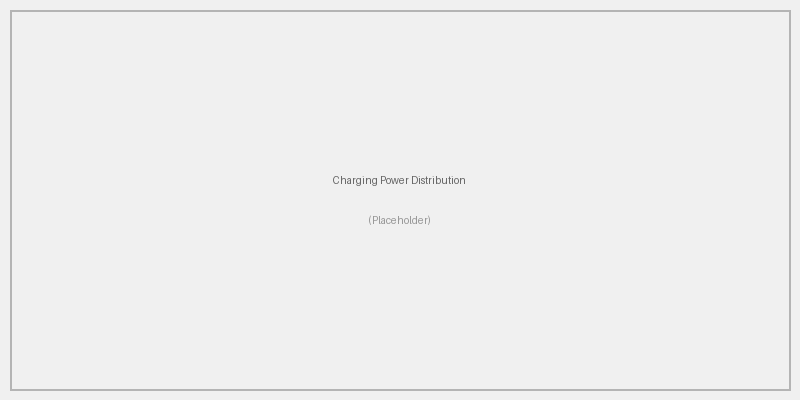
\includegraphics[width=0.8\textwidth]{figures/charging_power_distribution.png}
    \caption{Distribution of charging power across hours (RL method)}
    \label{fig:app_charging_dist}
\end{figure}

\subsection{Price vs. Charging Correlation}

\begin{figure}[H]
    \centering
    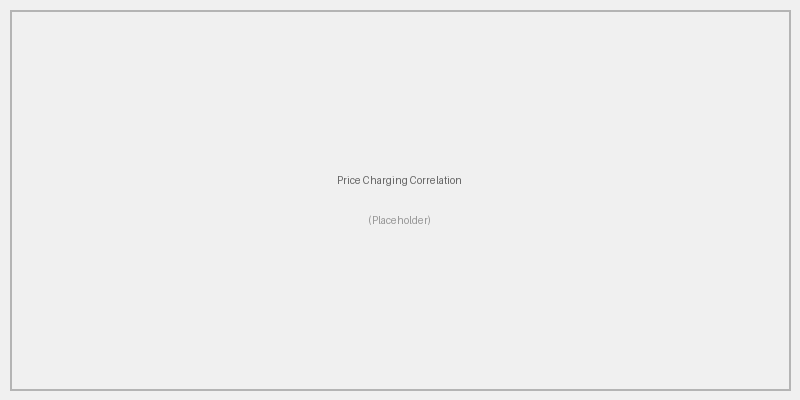
\includegraphics[width=0.8\textwidth]{figures/price_charging_correlation.png}
    \caption{Correlation between electricity price and charging activity}
    \label{fig:app_price_correlation}
\end{figure}

\subsection{Solar Utilization Breakdown}

\begin{figure}[H]
    \centering
    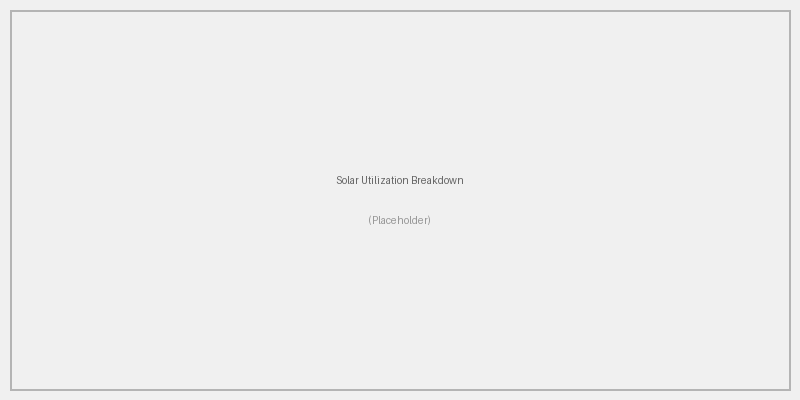
\includegraphics[width=0.8\textwidth]{figures/solar_utilization_breakdown.png}
    \caption{Solar energy allocation: Building vs. EV charging}
    \label{fig:app_solar_breakdown}
\end{figure}

\section{Computational Performance}
\label{app:computation}

\subsection{Execution Time Breakdown}

\begin{table}[H]
\centering
\caption{Detailed computational performance metrics}
\label{tab:app_computation}
\begin{tabular}{@{}lcccc@{}}
\toprule
\textbf{Algorithm} & \textbf{Training (s)} & \textbf{Per-Hour Exec (ms)} & \textbf{Memory (MB)} & \textbf{CPU Cores} \\
\midrule
Simple & 0 & [XX] & [XX] & 1 \\
RL (Q-Learning) & [XXX.X] & [XX] & [XXX] & 1 \\
\bottomrule
\end{tabular}
\end{table}

\subsection{Scalability Analysis}

\begin{table}[H]
\centering
\caption{Execution time vs. fleet size (seconds)}
\label{tab:app_scalability}
\begin{tabular}{@{}lccccc@{}}
\toprule
\textbf{Fleet Size} & \textbf{Simple} & \textbf{RL} \\
\midrule
5 & [X.X] & [XX.X] \\
10 & [X.X] & [XXX.X] \\
15 & [X.X] & [XXX.X] \\
20 & [X.X] & [XXX.X] \\
25 & [X.X] & [XXX.X] \\
\bottomrule
\end{tabular}
\end{table}

\section{Data Sources and References}
\label{app:data_sources}

\subsection{Building Consumption Data}

\textbf{Source:} ELMAS (European Load Model for Aggregated Sectors) dataset -- Office cluster \#5

\textbf{Description:}
\begin{itemize}
    \item Building type: Office/Commercial
    \item Source files: \texttt{Time\_series\_18\_clusters.csv}, \texttt{Annual\_energy\_time\_series.csv}, \texttt{Nb\_customers\_time\_series.csv}
    \item Target energy: 58,831~kWh/year (75th percentile of per-customer distribution)
    \item Measurement period: 2018 (8,736 hourly data points)
    \item Temporal resolution: 1 hour
    \item Data processing: Cluster profile scaled to target energy, stochastic variability applied ($\sigma_d = 0.08$, $\sigma_h = 0.03$), re-normalized to preserve annual total
    \item Output file: \texttt{office\_single\_building\_timeseries.csv}
\end{itemize}

\subsection{Solar PV Module Reference}

\textbf{Product:} JA Solar DeepBlue 3.0 Pro --- JAM54S31-405/MR~\cite{ja_solar_deepblue}

\textbf{Key specifications:}
\begin{table}[H]
\centering
\caption{JA Solar DeepBlue 3.0 Pro module specifications}
\label{tab:app_ja_solar}
\begin{tabular}{@{}lll@{}}
\toprule
\textbf{Parameter} & \textbf{Value} & \textbf{Unit} \\
\midrule
Rated power (Pmax, STC) & 405 & Wp \\
Module efficiency & 20.7 & \% \\
Cell type & Monocrystalline PERC & --- \\
Cell configuration & 54 cells (half-cut) & --- \\
Open-circuit voltage (Voc) & 37.20 & V \\
Short-circuit current (Isc) & 13.86 & A \\
Voltage at Pmax (Vmpp) & 31.10 & V \\
Current at Pmax (Impp) & 13.02 & A \\
Temperature coefficient (Pmax) & $-$0.35 & \%/°C \\
Dimensions (H $\times$ W $\times$ D) & 1722 $\times$ 1134 $\times$ 30 & mm \\
Module area & 1.953 & m\textsuperscript{2} \\
Weight & 21.8 & kg \\
Product warranty & 12 & years \\
Linear power warranty & 25 & years \\
\bottomrule
\end{tabular}
\end{table}

\textbf{System sizing:}
\begin{itemize}
    \item Number of modules: 74 ($74 \times 405\,\text{Wp} = 29{,}970\,\text{W} \approx 30\,\text{kW}$)
    \item Total module area: $74 \times 1.953\,\text{m}^2 = 144.5\,\text{m}^2 \approx 150\,\text{m}^2$
    \item Simulation uses rounded values: 150~m\textsuperscript{2} panel area, 20\% system efficiency, 30~kW peak
\end{itemize}

\subsection{Building Battery Reference}

\textbf{Product:} BYD Battery-Box Premium HVM~\cite{byd_batterybox}

\textbf{Key specifications:}
\begin{table}[H]
\centering
\caption{BYD Battery-Box Premium HVM specifications}
\label{tab:app_byd_battery}
\begin{tabular}{@{}lll@{}}
\toprule
\textbf{Parameter} & \textbf{Value} & \textbf{Unit} \\
\midrule
Cell chemistry & LiFePO\textsubscript{4} (LFP, cobalt-free) & --- \\
Module capacity & 2.76 & kWh \\
Module nominal voltage & 51.2 & V \\
Modules per tower & 3--8 & --- \\
Tower capacity range & 8.28--22.08 & kWh \\
Max parallel towers & 3 (per inverter) & --- \\
Round-trip efficiency & $\geq$\,96 (HTW Berlin cert.) & \% \\
Max output current & 50 & A \\
Peak output current & 75 (3~s) & A \\
Operating temperature & $-$10 to +50 & °C \\
Protection rating & IP55 & --- \\
Warranty & 10 & years \\
\bottomrule
\end{tabular}
\end{table}

\textbf{System sizing:}
\begin{itemize}
    \item Configuration: 4 $\times$ HVM~19.3 towers (7 modules each, multi-inverter setup)
    \item Total capacity: $4 \times 19.32\,\text{kWh} = 77.3\,\text{kWh} \approx 80\,\text{kWh}$
    \item Total max discharge power: $\approx$\,50~kW
    \item Simulation uses a conservative 95\% round-trip efficiency (vs.\ manufacturer-rated $\geq$\,96\%) to account for system-level losses including inverter and BMS overhead
\end{itemize}

\subsection{PVGIS Irradiance Data}

\textbf{Source:} European Commission Joint Research Centre - PVGIS

\textbf{Access:} \url{https://re.jrc.ec.europa.eu/pvg_tools/en/}

\textbf{Parameters:}
\begin{itemize}
    \item Location: Paris, France --- 48.857°N, 2.352°E (elevation 32~m)
    \item Database: PVGIS-SARAH3
    \item Plane orientation: Azimuth 0° (south-facing), Tilt 37° (site-optimum)
    \item Date: March 12, 2018
    \item Variables: Global irradiance on inclined plane $G(i)$ [W/m\textsuperscript{2}], sun height $H_{sun}$ [°], air temperature $T_{2m}$ [°C], wind speed $WS_{10m}$ [m/s]
    \item Peak irradiance (March 12): 487~W/m\textsuperscript{2} at 15:00
    \item Daily irradiation (March 12): 1{,}958~Wh/m\textsuperscript{2}
\end{itemize}

\subsection{Electricity Price Data}

\textbf{Source:} ENTSO-E Transparency Platform~\cite{entsoe_transparency}, cross-validated via Fraunhofer ISE Energy-Charts API~\cite{energy_charts}

\textbf{Access:}
\begin{itemize}
    \item ENTSO-E Transparency Platform: \url{https://transparency.entsoe.eu/}
    \item Energy-Charts API: \url{https://api.energy-charts.info/price?bzn=FR&start=2018-03-12T00:00&end=2018-03-12T23:59}
\end{itemize}

\textbf{Description:}
\begin{itemize}
    \item Market: EPEX SPOT -- French bidding zone (FR)~\cite{epex_spot}
    \item Price type: Day-ahead wholesale market (SDAC auction clearing price)
    \item Date: March 12, 2018
    \item Currency: EUR (€)
    \item Original unit: EUR/MWh (converted to EUR/kWh by dividing by 1000)
    \item Daily average: 38.67~EUR/MWh (0.039~EUR/kWh)
    \item Daily range: 9.56--62.00~EUR/MWh
    \item Minimum: 9.56~EUR/MWh at 03:00 (off-peak, nuclear baseload)
    \item Maximum: 62.00~EUR/MWh at 18:00 (evening peak)
    \item V2G sell-back price: 80\% of purchase price (accounts for grid fees, aggregator margin, and balancing costs)
    \item License: CC BY 4.0 (Energy-Charts data from Bundesnetzagentur / SMARD.de)
\end{itemize}

\section{Validation and Verification}
\label{app:validation}

\subsection{Unit Test Results}

\begin{table}[H]
\centering
\caption{Unit test coverage and results}
\label{tab:app_tests}
\begin{tabular}{@{}lcc@{}}
\toprule
\textbf{Test Module} & \textbf{Tests Passed} & \textbf{Coverage (\%)} \\
\midrule
test\_building.py & [XX]/[XX] & [XX]\% \\
test\_electric\_vehicle.py & [XX]/[XX] & [XX]\% \\
test\_grid.py & [XX]/[XX] & [XX]\% \\
test\_multi\_ev\_charging\_system.py & [XX]/[XX] & [XX]\% \\
test\_multi\_ev\_v2g\_charging\_system.py & [XX]/[XX] & [XX]\% \\
\midrule
\textbf{Total} & \textbf{[XXX]/[XXX]} & \textbf{[XX]\%} \\
\bottomrule
\end{tabular}
\end{table}

\subsection{Energy Balance Verification}

Verification that energy is conserved in all simulations:

\begin{equation}
\sum_{t=0}^{23} \left[ C_b(t) + \sum_{i=1}^{15} E_{charge}^i(t) \right] = \sum_{t=0}^{23} \left[ P_{solar}(t) + E_{grid}(t) + \sum_{i=1}^{15} E_{discharge}^i(t) \right]
\end{equation}

\textbf{Verification results:}
\begin{itemize}
    \item Energy balance error: < 0.01 kWh (numerical precision)
    \item All simulations pass energy conservation check
\end{itemize}

\section{Reproducibility Checklist}
\label{app:reproducibility_data}

To ensure reproducibility of results:

\begin{enumerate}
    \item \textbf{Software versions:}
    \begin{itemize}
        \item Python: 3.9.x or higher
        \item NumPy: 1.21.0
        \item Matplotlib: 3.4.0
        \item PuLP: 2.5.0
    \end{itemize}
    
    \item \textbf{Random seeds:}
    \begin{itemize}
        \item NumPy: \texttt{np.random.seed(42)}
        \item Python: \texttt{random.seed(42)}
        \item TensorFlow: \texttt{tf.random.set\_seed(42)}
    \end{itemize}
    
    \item \textbf{Data files:}
    \begin{itemize}
        \item All data files included in repository
        \item MD5 checksums provided for verification
    \end{itemize}
    
    \item \textbf{Configuration:}
    \begin{itemize}
        \item Exact configuration files preserved
        \item All parameters documented
    \end{itemize}
\end{enumerate}

\section{Hardware Specifications}
\label{app:hardware}

Simulations were conducted on:

\begin{table}[H]
\centering
\caption{Hardware specifications}
\label{tab:app_hardware}
\begin{tabular}{@{}ll@{}}
\toprule
\textbf{Component} & \textbf{Specification} \\
\midrule
CPU & [Processor model] \\
RAM & [XX] GB \\
GPU & N/A \\
Operating System & [OS name and version] \\
Python Version & 3.9.x \\
\bottomrule
\end{tabular}
\end{table}


\end{document}
